%%%%%%%%%%%%%%%%%%%%%%%%%%%%%%%%%%%%%%%%%
% Jacobs Landscape Poster
% LaTeX Template
% Version 1.1 (14/06/14)
%
% Created by:
% Computational Physics and Biophysics Group, Jacobs University
% https://teamwork.jacobs-university.de:8443/confluence/display/CoPandBiG/LaTeX+Poster
% 
% Further modified by:
% Nathaniel Johnston (nathaniel@njohnston.ca)
%
% This template has been downloaded from:
% http://www.LaTeXTemplates.com
%
% License:
% CC BY-NC-SA 3.0 (http://creativecommons.org/licenses/by-nc-sa/3.0/)
%
%%%%%%%%%%%%%%%%%%%%%%%%%%%%%%%%%%%%%%%%%

%----------------------------------------------------------------------------------------
%	PACKAGES AND OTHER DOCUMENT CONFIGURATIONS
%----------------------------------------------------------------------------------------

%\documentclass[final]{beamer}
\documentclass[final]{beamer}

\usepackage[scale=1.24]{beamerposter} % Use the beamerposter package for laying out the poster

\usepackage[utf8]{inputenc}
\usepackage[english]{babel}

%\usepackage{wrapfig}
%\usepackage{fancyhdr}
\usepackage{float}
 %\usepackage{graphicx}
%\usepackage{subfig}
\usepackage{tikz}
\usepackage{soul}
\usetikzlibrary{spy}

\usepackage[position=t,singlelinecheck=off]{subfig}
\usepackage{caption}

\renewcommand\thesubfigure{\alph{subfigure}}

\usetheme{confposter} % Use the confposter theme supplied with this template

\setbeamercolor{block title}{fg=dgreen,bg=white} % Colors of the block titles
\setbeamercolor{block body}{fg=black,bg=white} % Colors of the body of blocks
\setbeamercolor{block alerted title}{fg=white,bg=dblue!70} % Colors of the highlighted block titles
\setbeamercolor{block alerted body}{fg=black,bg=dblue!10} % Colors of the body of highlighted blocks
% Many more colors are available for use in beamerthemeconfposter.sty

%\setbeamercolor{bibliography entry author}{fg=red}
%\setbeamercolor{bibliography entry title}{fg=blue} 
\setbeamercolor{bibliography entry location}{fg=DarkGray} 
%\setbeamercolor{bibliography entry note}{fg=cyan} 

\setbeamertemplate{caption}[numbered] % Figure numbering 

%-----------------------------------------------------------
% Define the column widths and overall poster size
% To set effective sepwid, onecolwid and twocolwid values, first choose how many columns you want and how much separation you want between columns
% In this template, the separation width chosen is 0.024 of the paper width and a 4-column layout
% onecolwid should therefore be (1-(# of columns+1)*sepwid)/# of columns e.g. (1-(4+1)*0.024)/4 = 0.22
% Set twocolwid to be (2*onecolwid)+sepwid = 0.464
% Set threecolwid to be (3*onecolwid)+2*sepwid = 0.708

\newlength{\sepwid}
\newlength{\onecolwid}
\newlength{\twocolwid}
\newlength{\threecolwid}
\setlength{\paperwidth}{1189mm} % A0 width: 46.8in
\setlength{\paperheight}{841mm} % A0 height: 33.1in
\setlength{\sepwid}{0.00\paperwidth} % Separation width (white space) between columns
\setlength{\onecolwid}{0.22\paperwidth} % Width of one column
\setlength{\twocolwid}{0.464\paperwidth} % Width of two columns
\setlength{\threecolwid}{0.708\paperwidth} % Width of three columns
\setlength{\topmargin}{-0.5in} % Reduce the top margin size
%-----------------------------------------------------------

\usepackage{graphicx}  % Required for including images

\usepackage{booktabs} % Top and bottom rules for tables

%----------------------------------------------------------------------------------------
%	TITLE SECTION 
%----------------------------------------------------------------------------------------

\title{Predicting I/O-performance in HPC using Artificial Neural Networks} % Poster title

\author{Jan Fabian Schmid and Julian Kunkel} % Author(s)

%\author{Jan Fabian Schmid \href{mailto:2schmid@informatik.uni-hamburg.de}{\textit{{\normalsize 2schmid@informatik.uni-hamburg.de}}}, Julian Kunkel \href{mailto:juliankunkel@googlemail.com}{\textit{{\normalsize juliankunkel@googlemail.com}}}} % Author(s)

\institute{Universität Hamburg} % Institution(s)

%\item \href{mailto:2schmid@informatik.uni-hamburg.de}{2schmid@informatik.uni-hamburg.de}
%\item \href{mailto:juliankunkel@googlemail.com}{juliankunkel@googlemail.com}

%----------------------------------------------------------------------------------------

\begin{document}
	
	\small

\addtobeamertemplate{block end}{}{\vspace*{2ex}} % White space under blocks
\addtobeamertemplate{block alerted end}{}{\vspace*{2ex}} % White space under highlighted (alert) blocks

\setlength{\belowcaptionskip}{2ex} % White space under figures
\setlength\belowdisplayshortskip{2ex} % White space under equations

\begin{frame}[t] % The whole poster is enclosed in one beamer frame

\begin{columns}[t] % The whole poster consists of three major columns, the second of which is split into two columns twice - the [t] option aligns each column's content to the top

\begin{column}{\sepwid}\end{column} % Empty spacer column

\setlength{\sepwid}{0.02\paperwidth} % Separation width (white space) between columns

\begin{column}{\onecolwid} % The first column

%----------------------------------------------------------------------------------------
%	GOALS
%----------------------------------------------------------------------------------------

	\small

\setbeamercolor{block title}{fg=dgreen,bg=white} % Colors of the block titles
\setbeamercolor{block body}{fg=black,bg=white} % Colors of the body of blocks
\setbeamercolor{block alerted title}{fg=white,bg=dblue!70} % Colors of the highlighted block titles
\setbeamercolor{block alerted body}{fg=black,bg=dblue!10} % Colors of the body of highlighted blocks
% Many more colors are available for use in beamerthemeconfposter.sty

\begin{alertblock}{Goals}
	
%The goals of this work were:

\begin{itemize}
\item Gain knowledge about the storage system of a super computer for the development of computational models and tools in the future.
\item Find a good model that is reliable in predicting performance of HPC-IO with sufficient quality.
\item Extract information about the I/O-paths the storage system used for measured file accesses.
\end{itemize}

\end{alertblock}

%----------------------------------------------------------------------------------------
%	INTRODUCTION
%----------------------------------------------------------------------------------------

\begin{block}{Introduction}
	
There is a need for tools that help users to implement efficient input/output (I/O) in their software.
Finding the best access parameters and patterns is difficult, mainly because of the use of complex parallel storage systems in HPC.
%Currently users have to optimize their programs at great expense to each system individually without much assistance.
For the development of tools, to support the implementation of efficient I/O, it is key to have a computational model of the storage system.\medskip

For single hard disk systems such a model can be derived analytically \cite{Ruemmler94anintroduction}, however for the complex storage system of a super computer these models become too difficult to configure \cite{DBLP:conf/npc/ZhangLZJC10}.
Therefore we tried to find a good predictor for I/O-performance using a machine learning approach with artificial neural networks (ANNs).
A hypothesis was then proposed: \textbf{The I/O-path significantly influences the time needed for a file access.}\medskip
%In particular the access time for a file access is more dependent on the I/O-path used in the storage system than on the access size for example.

We used ANNs with different input information for the prediction of access times to test our hypothesis.
For the use of I/O-paths as input information for the ANNs we developed a method to approximate the different I/O-paths the storage system used during a benchmark-test.
This method utilizes error classes.

\end{block}

%------------------------------------------------

%\begin{figure}
%\includegraphics[width=0.8\linewidth]{placeholder.jpg}
%\caption{Figure caption}
%\end{figure}

%----------------------------------------------------------------------------------------

\begin{block}{Artificial Neural Networks}
	
	ANNs are bio-inspired function approximators.
	
	%\begin{wrapfigure}{r}{0.6\textwidth}
	%	\begin{center}
	%		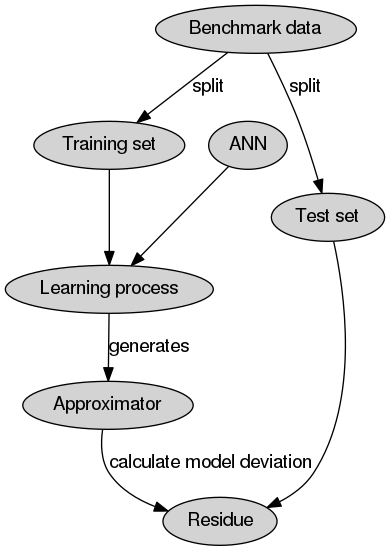
\includegraphics[height=1\textwidth]{src/tupel1.png}
	%	\end{center}
	%	\caption{G}
	%	\label{fig:evo}
	%\end{wrapfigure}
	
	An ANN is able to approximate a function that maps given input vectors on their associated output vectors.
	This is done by adapting the connection weights in the network using gradient decent during a supervised learning process (backpropagation).
	With appropriate topology \textbf{ANNs are able to approximate any continuous functions} on compact subsets of $\mathbb{R}^n$ \cite{cybenko:mcss}.
	
%	\begin{figure}
%	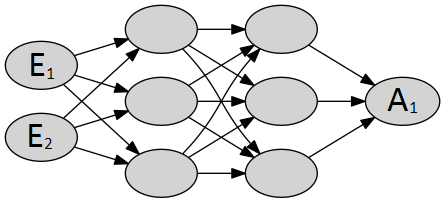
\includegraphics[height=0.3\linewidth]{src/netz.png}
%	\caption{small feedforward-network}
%	\label{netz}
%	\end{figure}
	
\end{block}

\end{column} % End of the first column

\begin{column}{\sepwid}\end{column} % Empty spacer column

\begin{column}{\onecolwid} % The sec column
	

\begin{block}{Model of the I/O-path}
	
	The processing of a file access in the storage system can be viewed using the I/O-path, which is \textbf{the path from the invoking processor to the storage medium that contains the data}.
	The resulting access time of the process then depends on the depth of this I/O-path, because storage media further along the path becomes increasingly slower.
	%the further the path leads into the storage system, the slower the storage media gets.
	While the first storage levels (Caches) are very quick to respond, the main memory is already magnitudes slower; the same applies for the step into the parallel storage system that is connected via network to the computer nodes. %\medskip
		
%	\begin{tikzpicture}[spy using outlines={circle,black,magnification=5,size=1.5cm, connect spies}]
%		\node {\pgfimage[width=.55\textwidth]{src/plot_SizeSorted_log_read_seq.png}};
%		\spy on (0,1) in node [left] at (10,1.25);
%	\end{tikzpicture}
	
	%\begin{tikzpicture}[spy using outlines={circle,black,magnification=2.5,size=4.5cm, connect spies}]
	%	\node {\pgfimage[interpolate=true,width=.55\textwidth]{src/plot_SizeSorted_log_read_seq.png}};
	%	\spy on (3.5,0.5) in node [left] at (14,1.25);
	%\end{tikzpicture}


%	\begin{figure}		
%		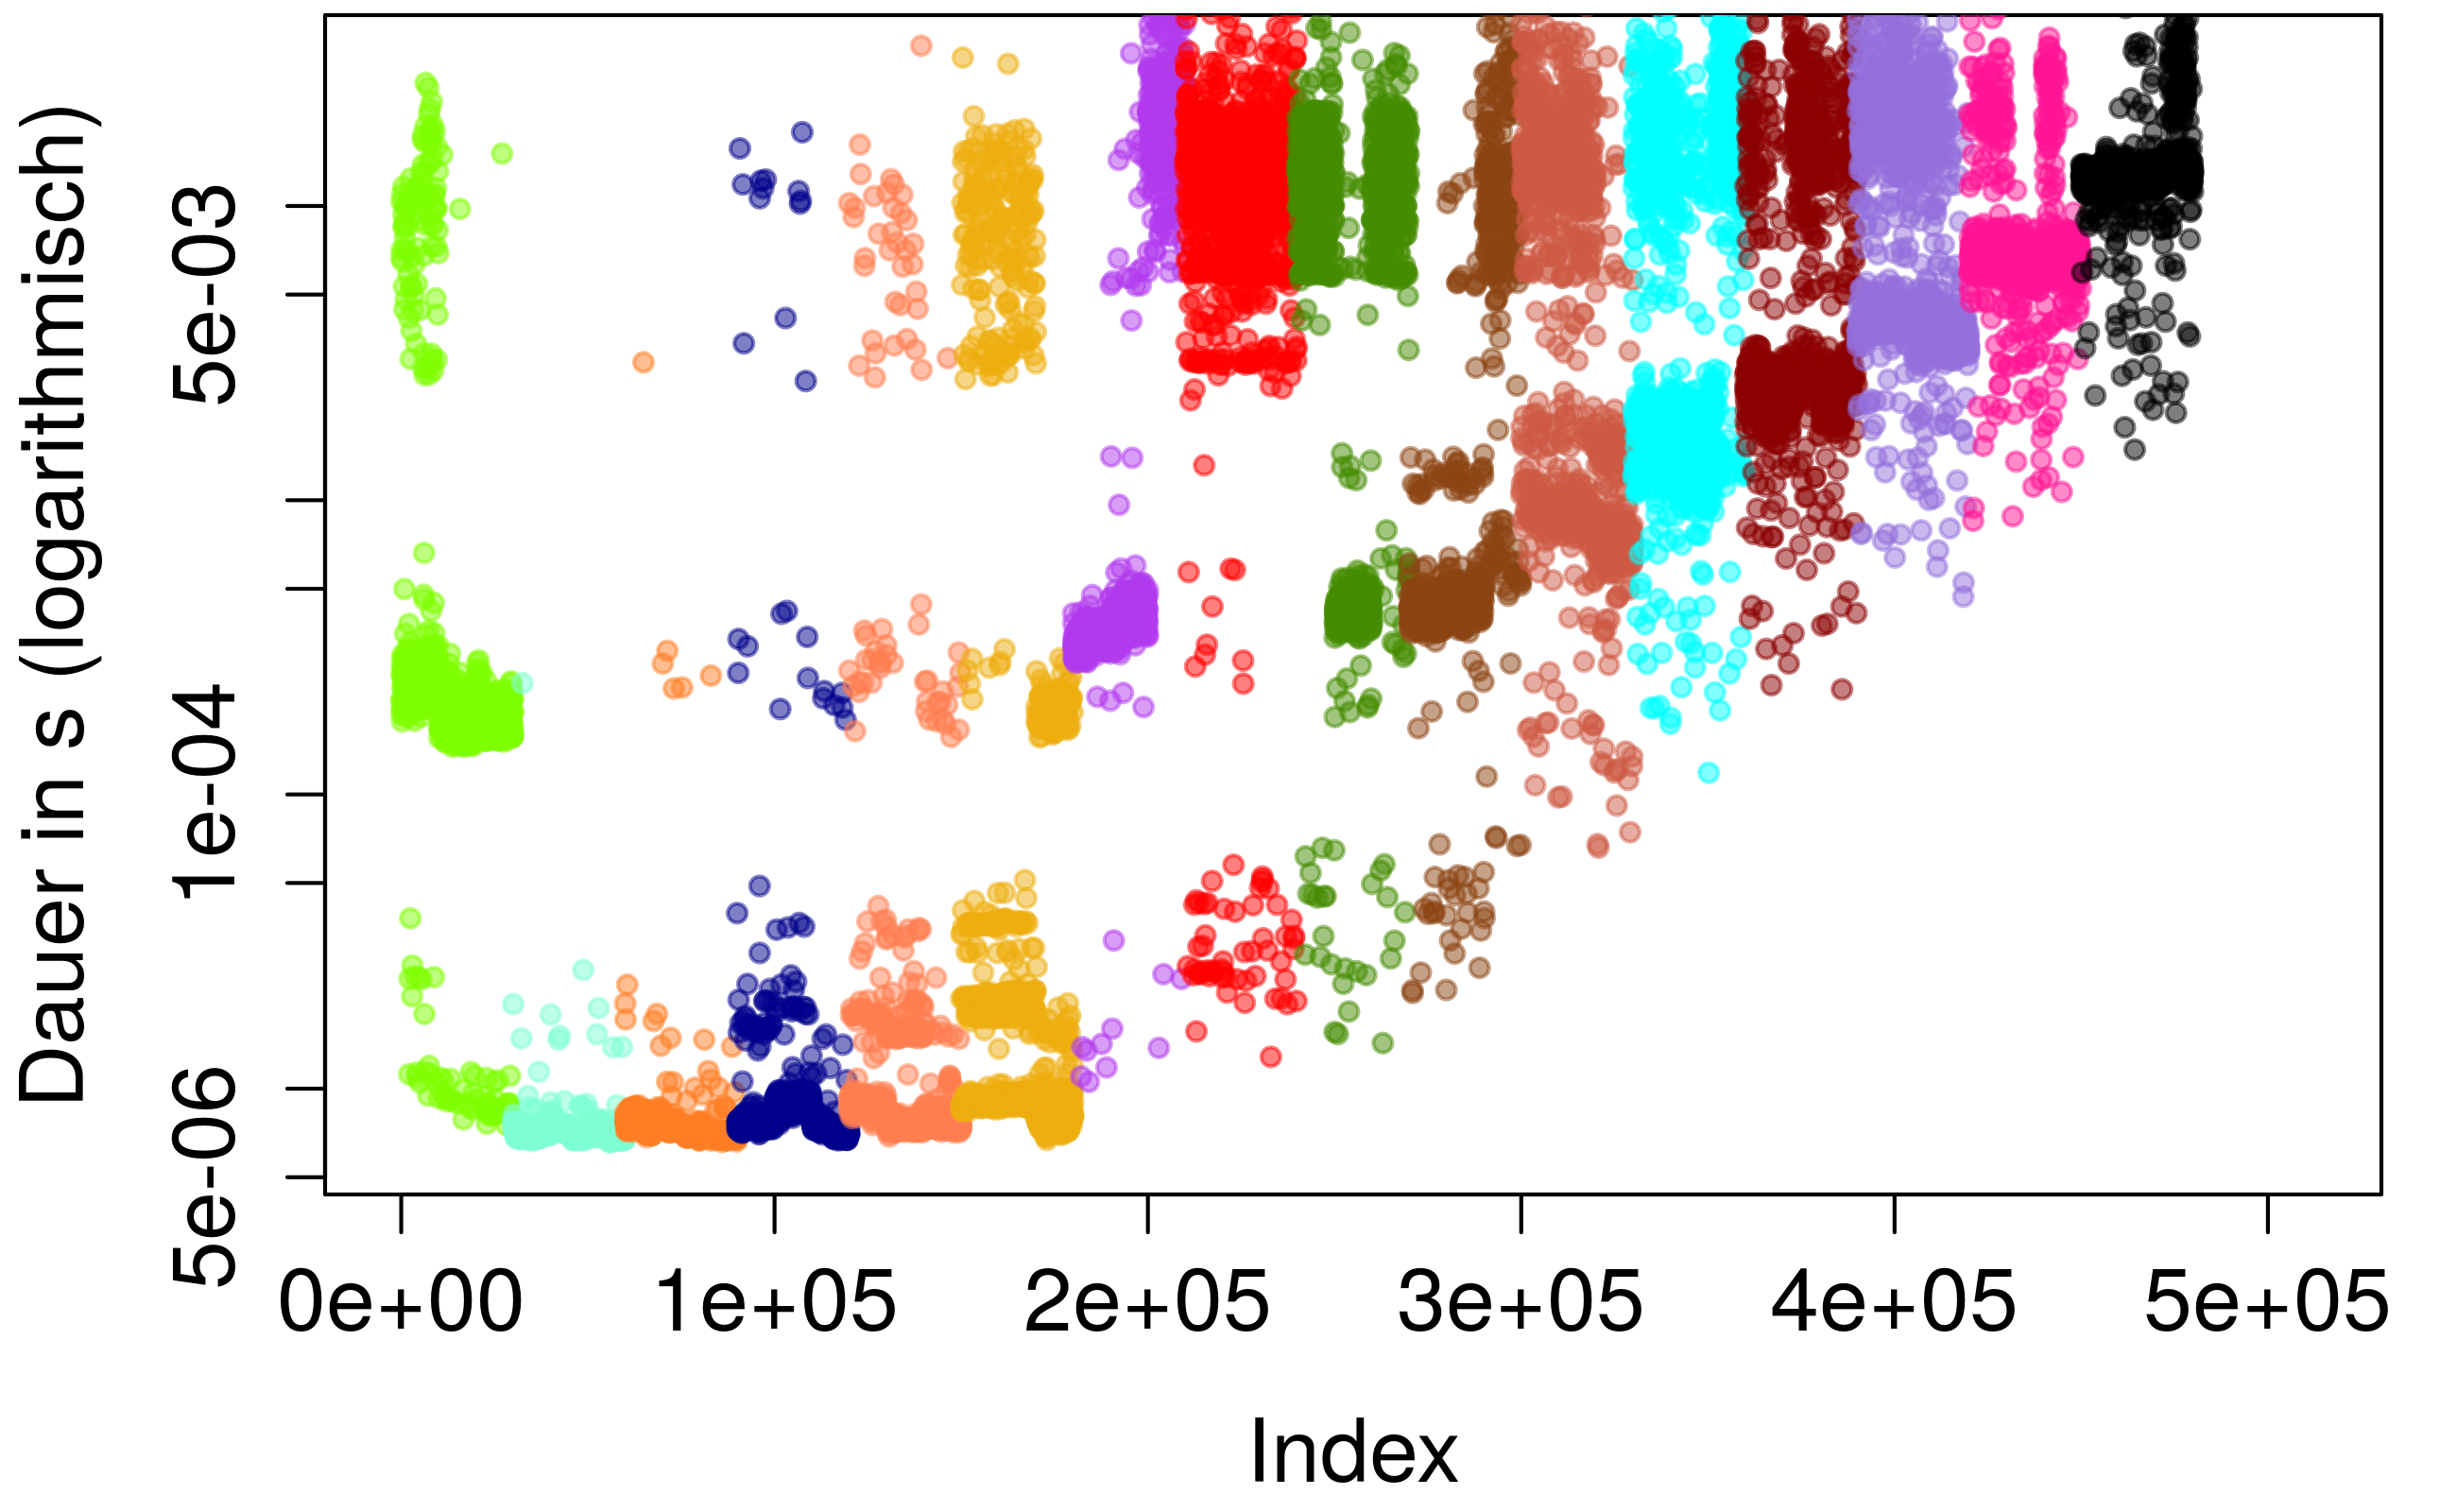
\includegraphics[width=0.7\linewidth]{src/plot_SizeSorted_log_read_rnd.png}
%		\vspace*{-0.5cm}
%		\caption{Access times of measurements with increasing access sizes. The sizes increase from left to right, all measurements with the same size have the same color.}
%		\label{read_rnd}
%	\end{figure}
	
	%\begin{figure}
	%	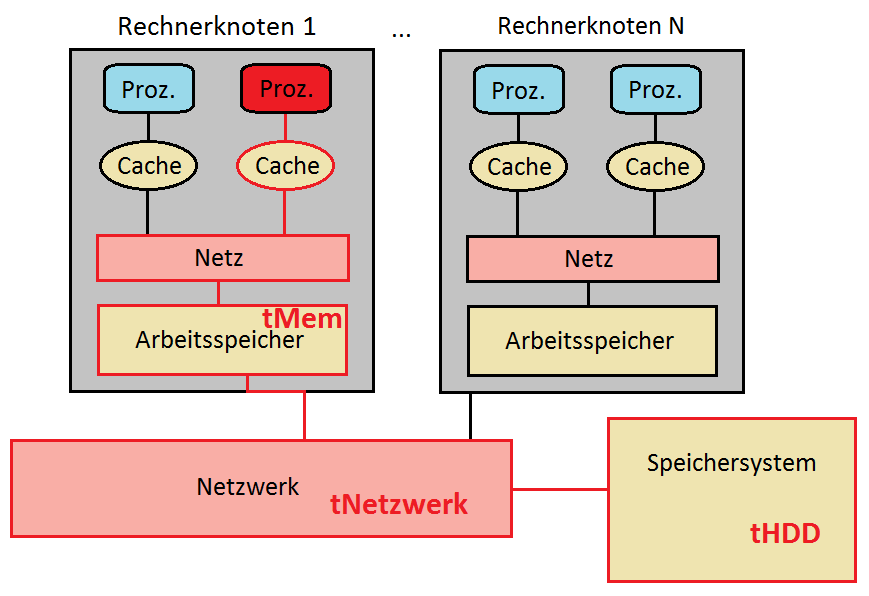
\includegraphics[width=1\linewidth]{src/rechnerknoten_ea_pfad.png}
	%	\caption{Sketch of the storage system in a super computer}
	%\end{figure}
	
\end{block}

%\vspace*{-2cm}
\begin{block}{Benchmark-Tests}
	
	The measurements were done on the super computer Mistral of the DKRZ (Deutsches Klimarechenzentrum).
	Mistral operates with the parallel distributed file system Lustre and consist of over 1500 computing nodes and 30 petabyte storage.
	\textbf{Two different use cases were tested: Sequential and random file access.}
	Access sizes varied from 1\,B to 16\,MiB.\medskip
	
	Our measurements showed, as can be seen in figure \ref{exploration}, that the access times increase with access sizes.
	However a phenomenon that can be explained with the I/O-path model can be seen as well: \textbf{Access times of measurements with equal parameter values are split into several groups of access times.}
	The used I/O-paths for the file accesses distinguishes these groups of measurements through a step in the magnitude of access time.
	%Different I/O-paths were used for file accesses in these groups, which led to a step in the magnitude of the access time. 
		
	\begin{figure}
		%\flushleft
		\captionsetup[subfigure]{margin={-0.4cm,0cm}}
		\subfloat[Sequential access pattern]{
			%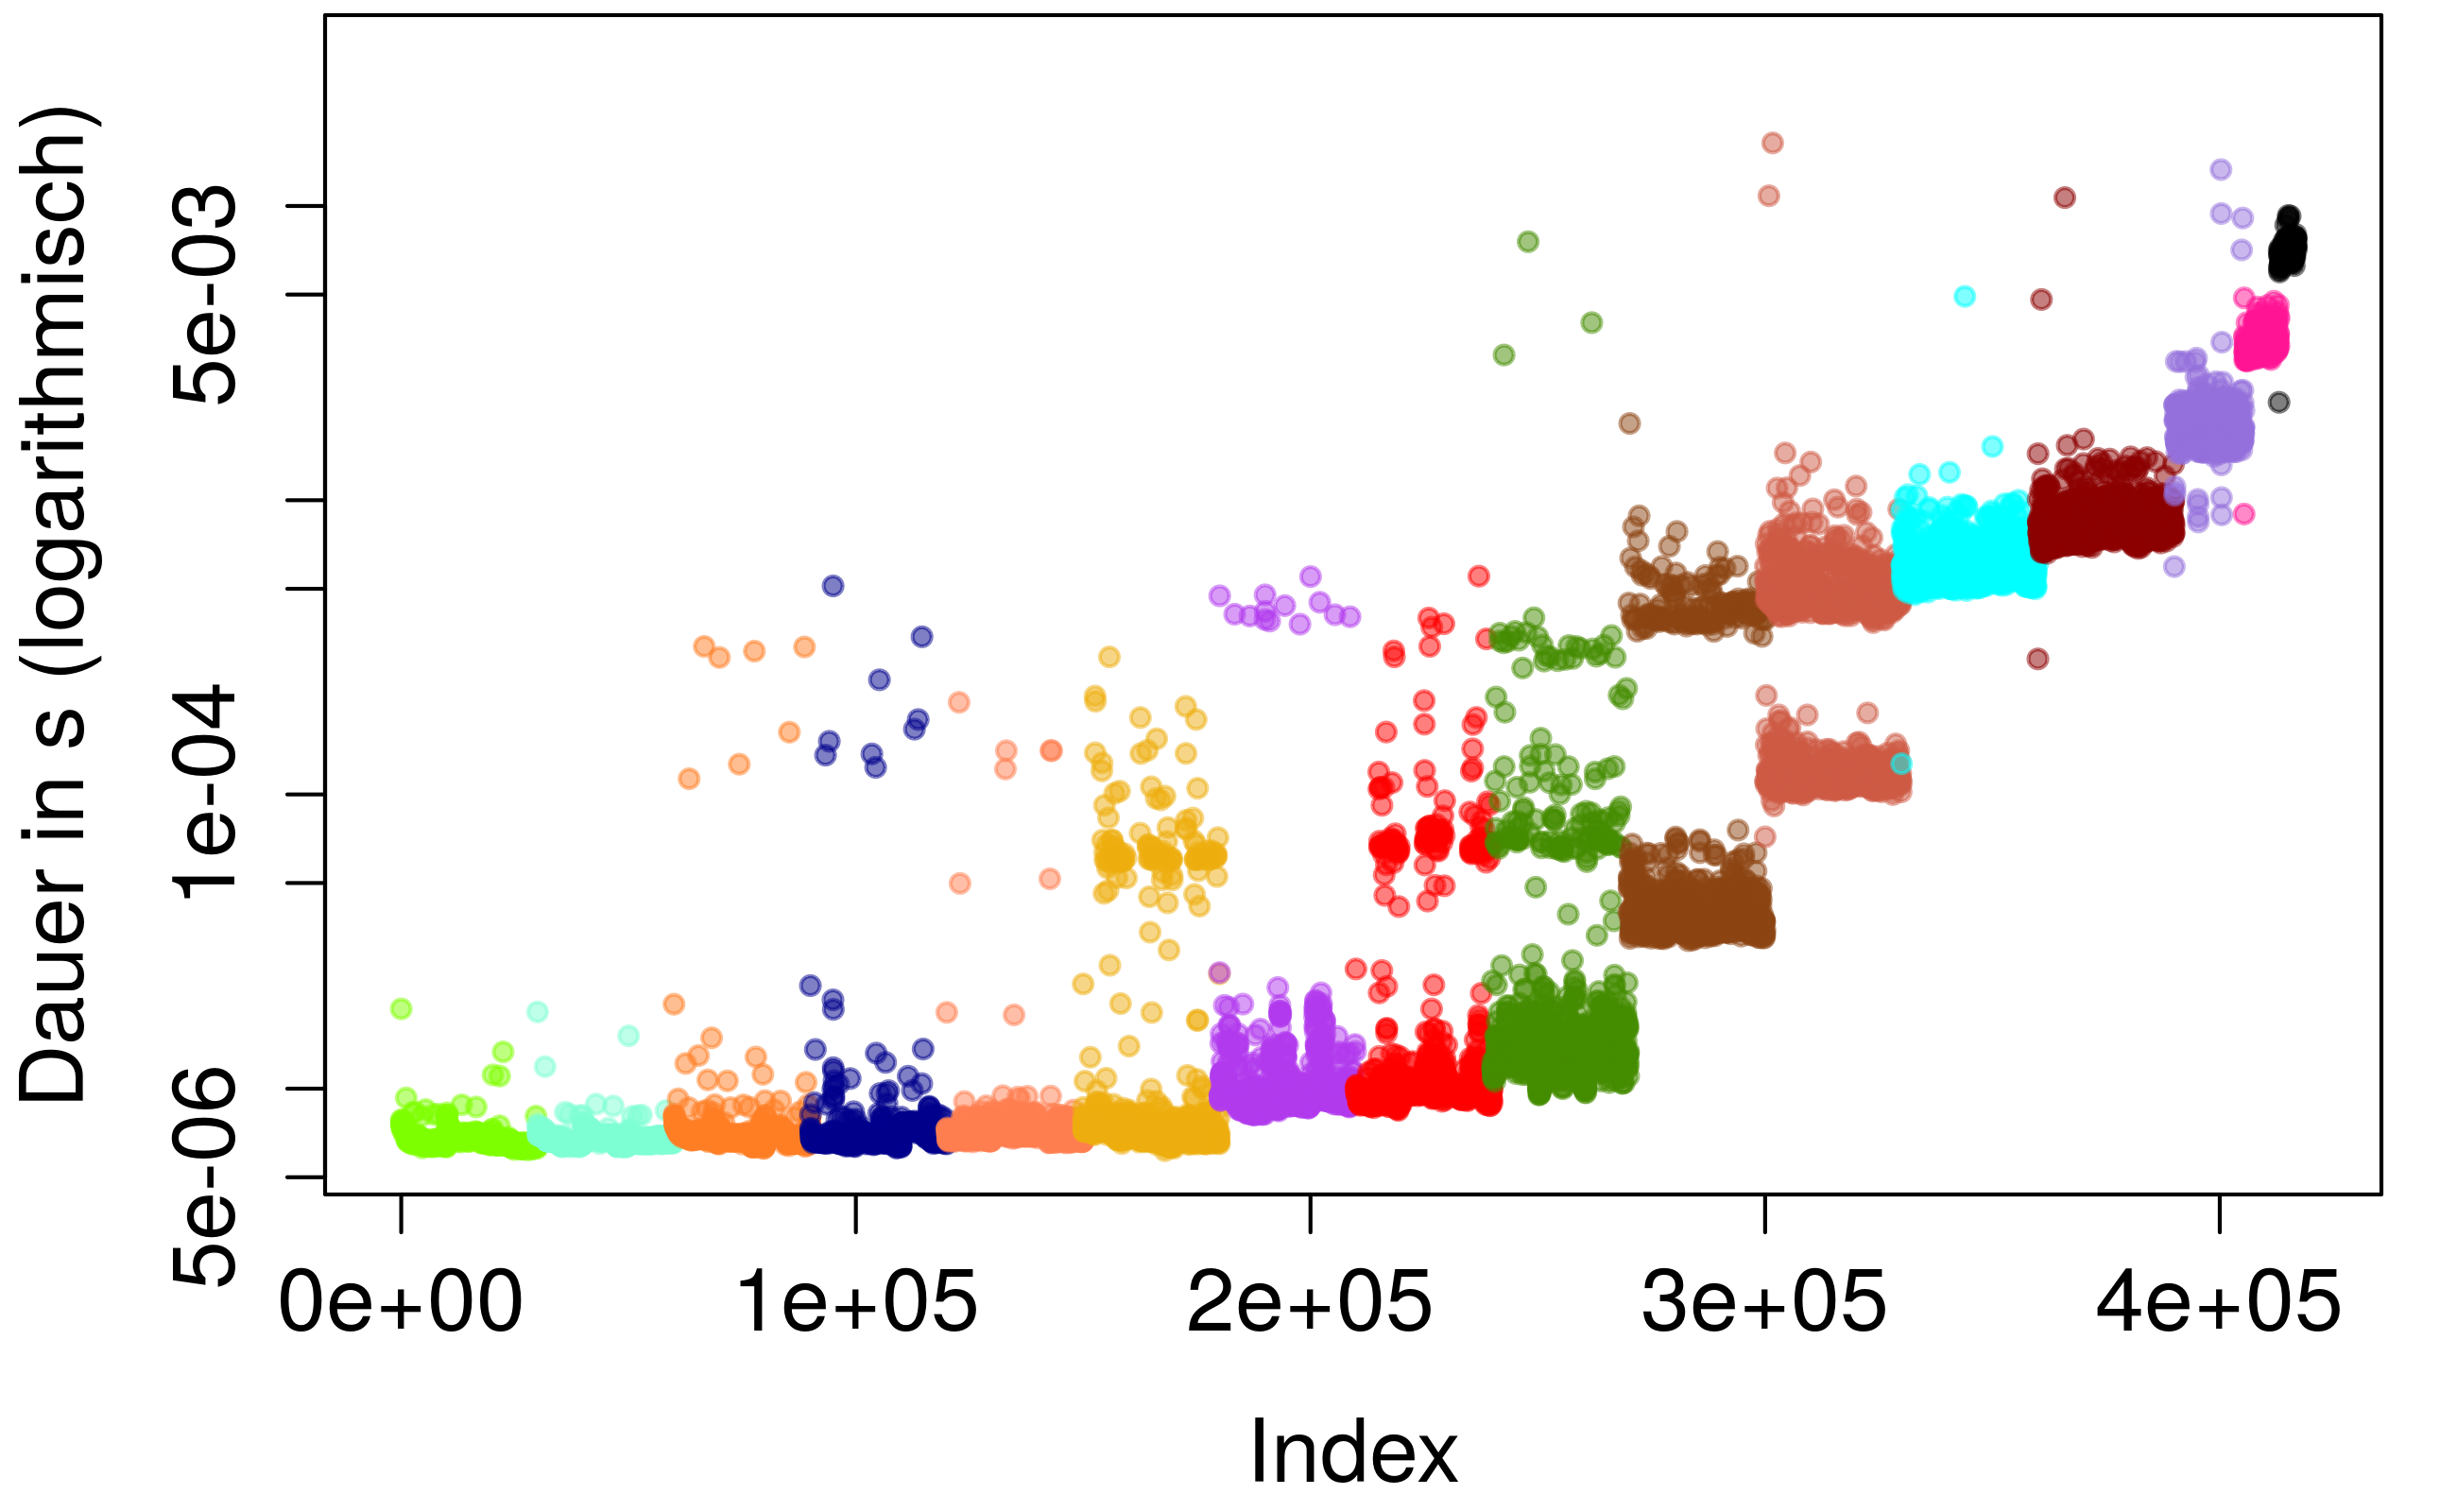
\includegraphics[width=.55\textwidth]{src/plot_SizeSorted_log_read_seq.png}
			\begin{tikzpicture}[spy using outlines={circle,black,magnification=2.2,size=4.5cm, connect spies}]
			\node {\pgfimage[interpolate=true,width=.53\textwidth]{src/plot_SizeSorted_log_read_seq.png}};
			%\draw (3.5,0.5) ellipse (1 and 1);
			\spy on (3.4,0.5) in node [left] at (14,1.25);
			\end{tikzpicture}
		}
		%\hfill
		\\
		\captionsetup[subfigure]{margin={-0.4cm,0cm}}
		\vspace*{0.25cm}	
		\hspace*{-7.365cm}		
		\subfloat[Random access pattern]{
			%\hspace*{-5cm}
			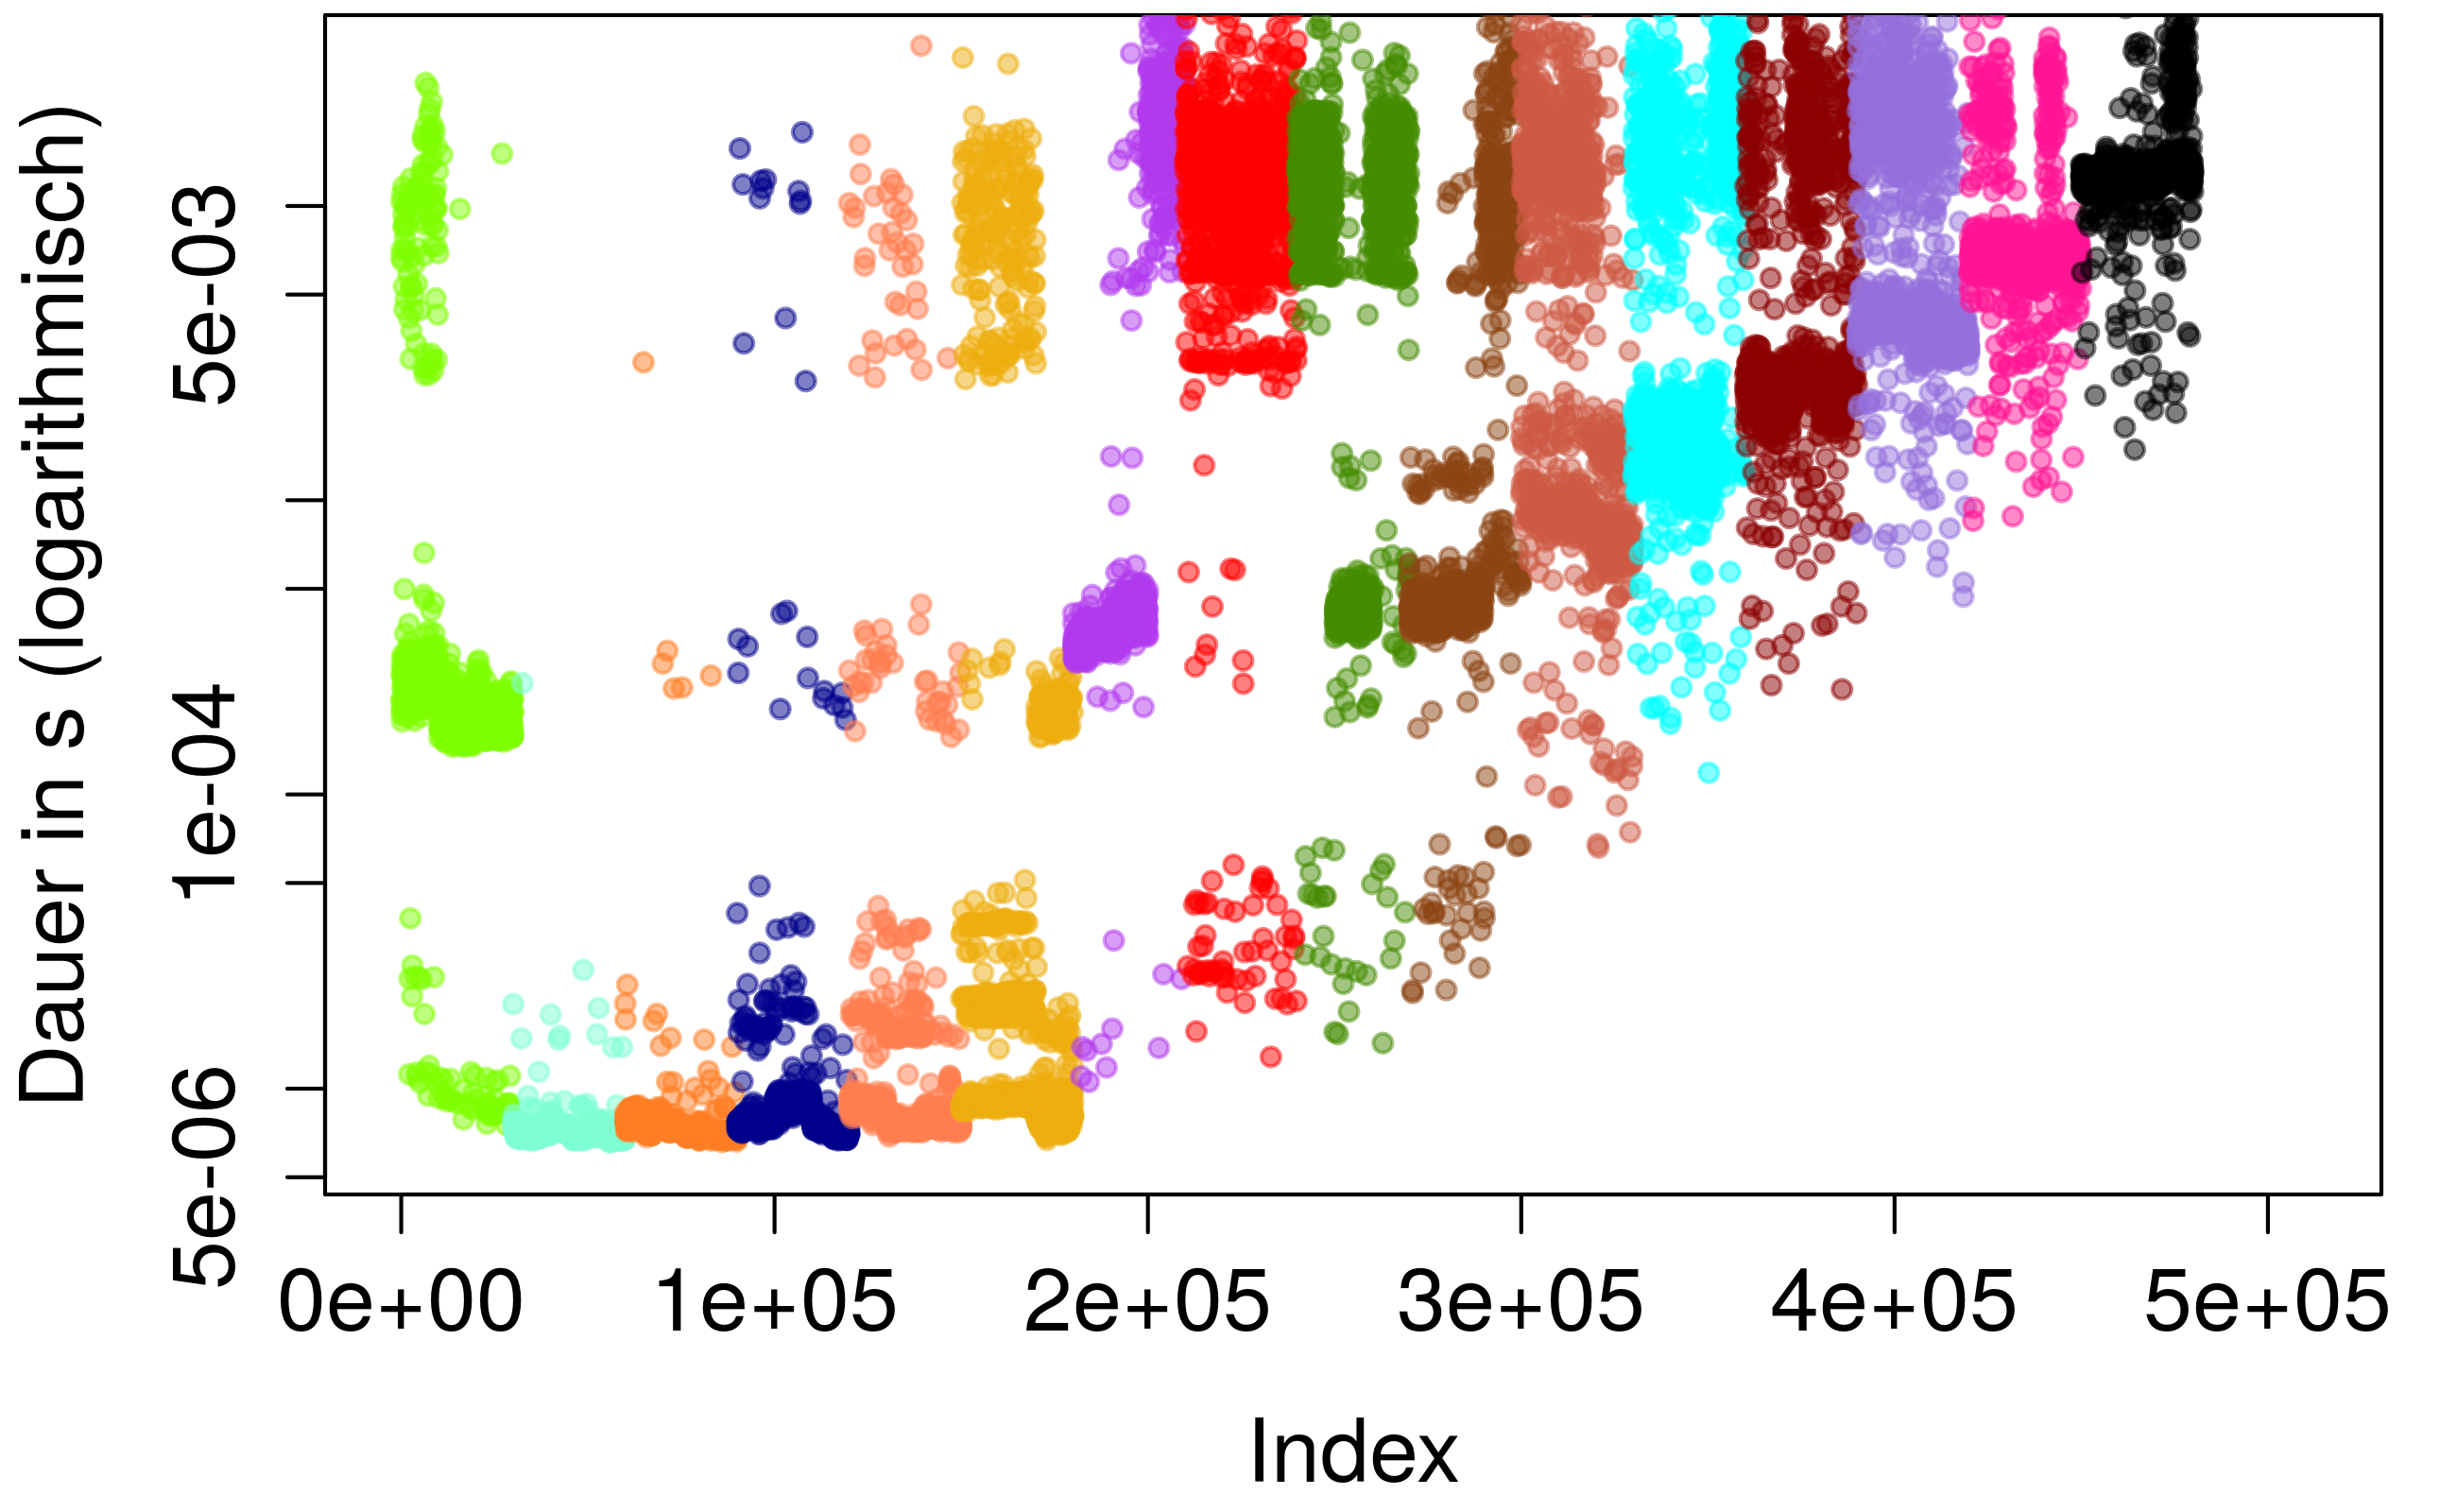
\includegraphics[width=.53\textwidth]{src/plot_SizeSorted_log_read_rnd.png}
		}
		\vspace*{-0.05cm}	
		\caption{Access times of measured file accesses. The access sizes increase from left to right, all measurements with equal parameter values have the same color. In the highlighted section the described step in the access time occurs.}
		\label{exploration}
	\end{figure} 
	
\end{block}
	
\end{column} % End of the sec column

\begin{column}{\sepwid}\end{column} % Empty spacer column

\begin{column}{\onecolwid} % The 3 column
	

\begin{block}{Models}
	
	Different models were used to predict access times of file accesses.
	As baseline model linear regression was used for a simple mapping of access size to access time.
	Additionally three \textbf{models with different input information utilizing ANNs were used}.
	Every ANN-model received information about access sizes, file offsets and access types as input.
	One ANN also received information about the past data throughputs of the system, which can be used to exploit time dependencies of the I/O-performance (see figure \ref{time_dep}). The last ANN received error classes as additional input.
	
	\begin{figure}
		\subfloat[In this sequence peaks in the access times occur regularly.]{
			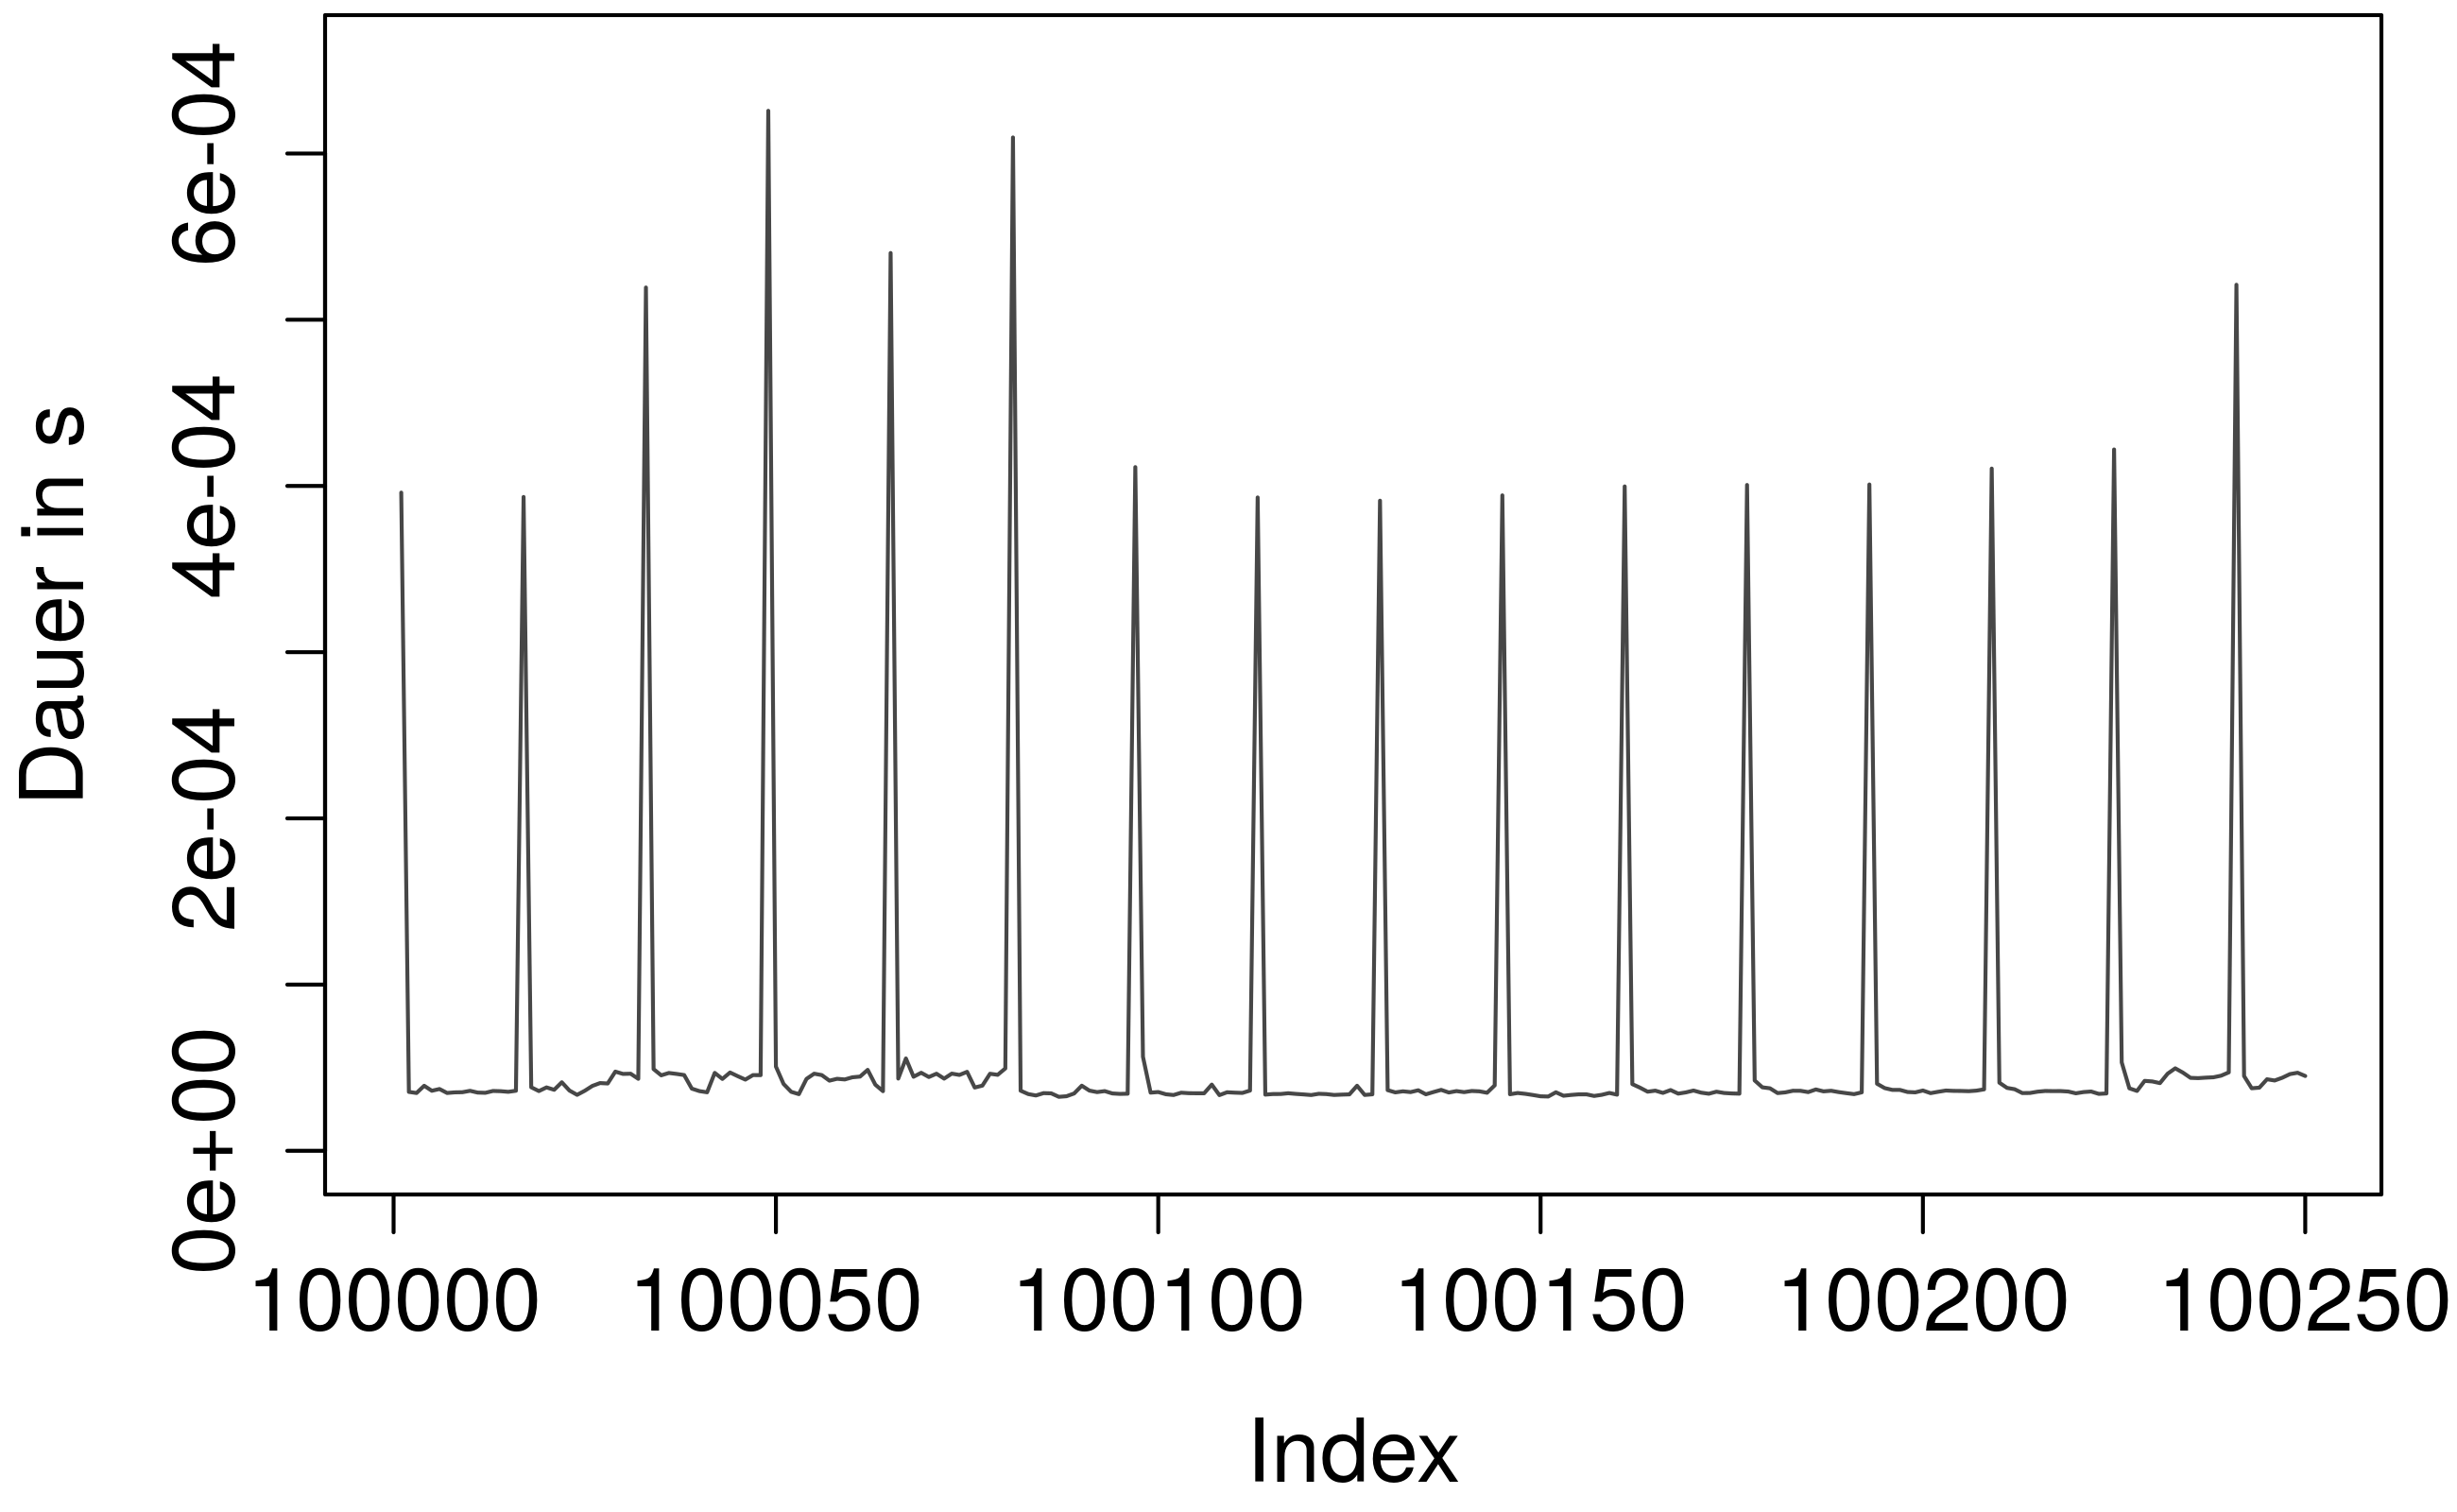
\includegraphics[width=.48\textwidth]{src/plot_From100001to100250_read_seq.png}
		}
		\hfill
		\subfloat[Exponential moving average in red to predict peaks.]{
			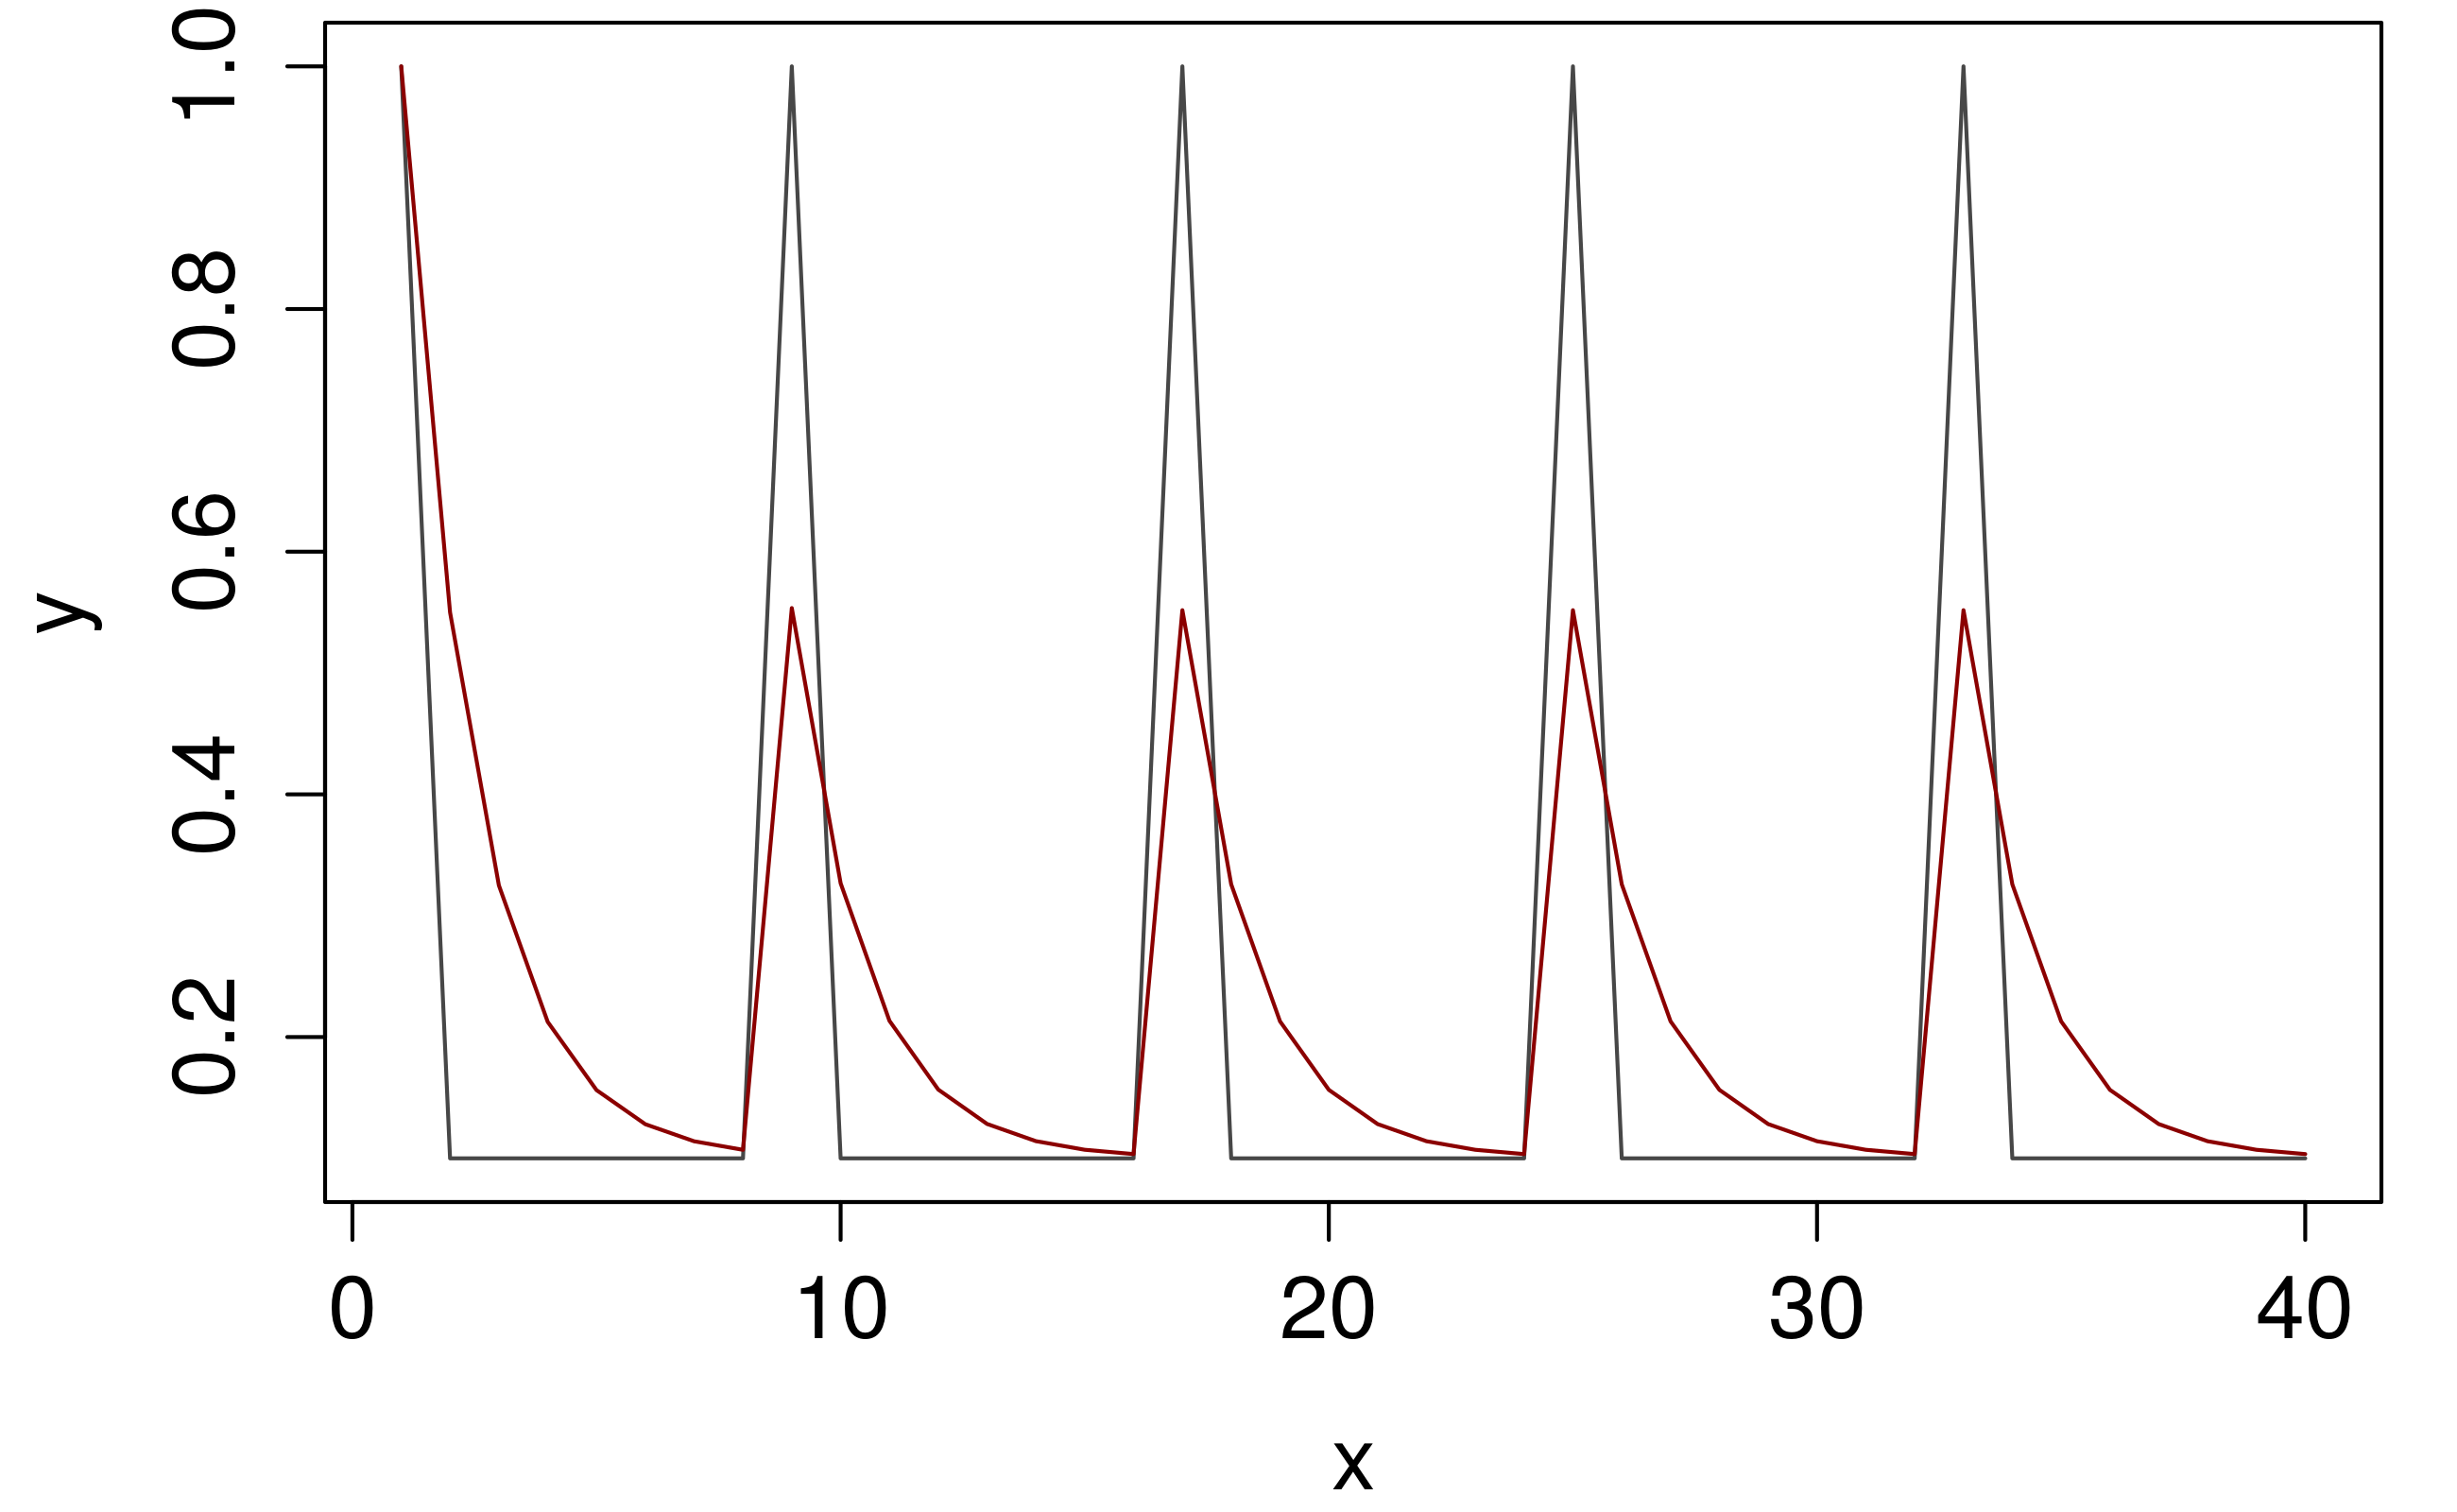
\includegraphics[width=.48\textwidth]{src/ema2.png}
		}	
		\caption{Time dependencies can be utilized for better access time predictions.}
		\label{time_dep}
	\end{figure} 
	
%		\begin{figure}
%			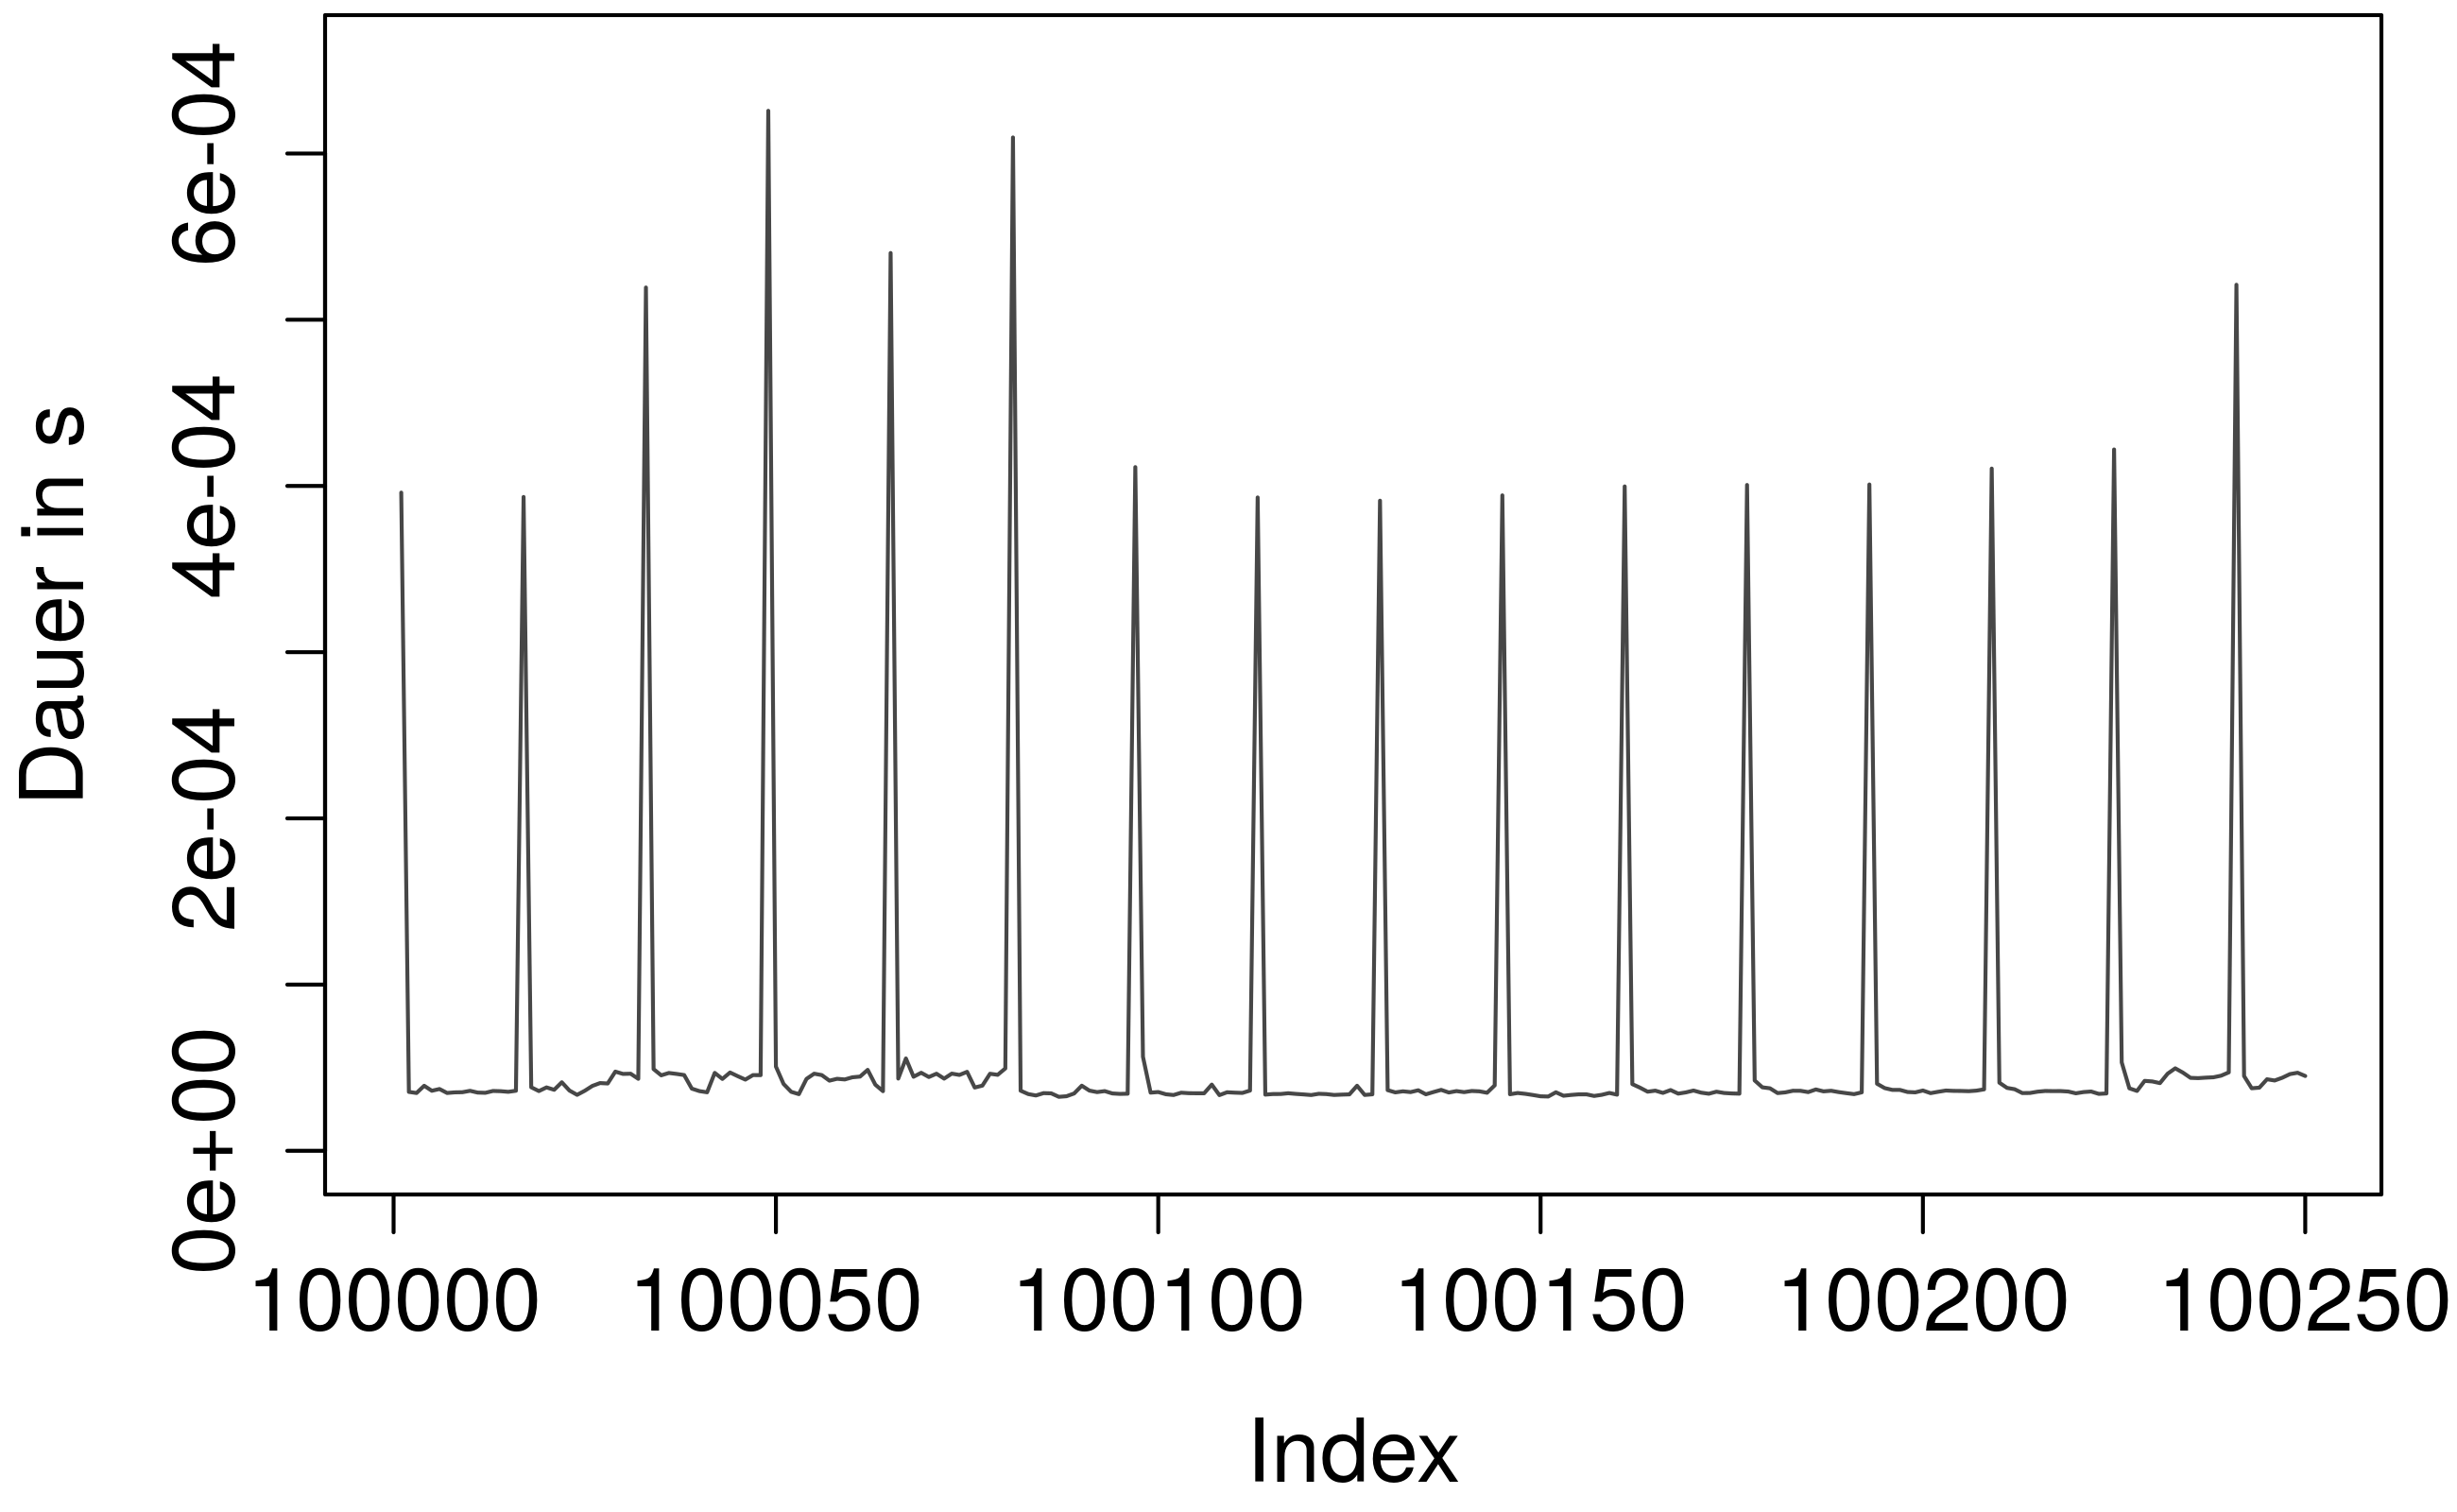
\includegraphics[width=0.7\linewidth]{src/plot_From100001to100250_read_seq.png}
%			\vspace*{-0.5cm}
%			\caption{A small sequence of file accesses with same parameters. Peaks in the access times occure regularly.}
%			\label{time_dep}
%		\end{figure}
	
\end{block}

\vspace*{-2cm}
\begin{block}{Error Classes}
	
The idea of error classes is based on the fact that \textbf{the residues of a simple model are characteristic for the groups of measurements with different typical access times} obeserved in figure \ref{exploration}. The residues therefore represent the I/O-paths used by the storage system for the corresponding file accesses. 
%Here a simple model is a model that doesn't discriminate measurements with similar parameters.
Error classes are then obtained by clustering the residues with a k-Means algorithm.

%	\begin{figure}
%		%\flushleft
%		%\subfloat[Sequential access pattern]{
%		%	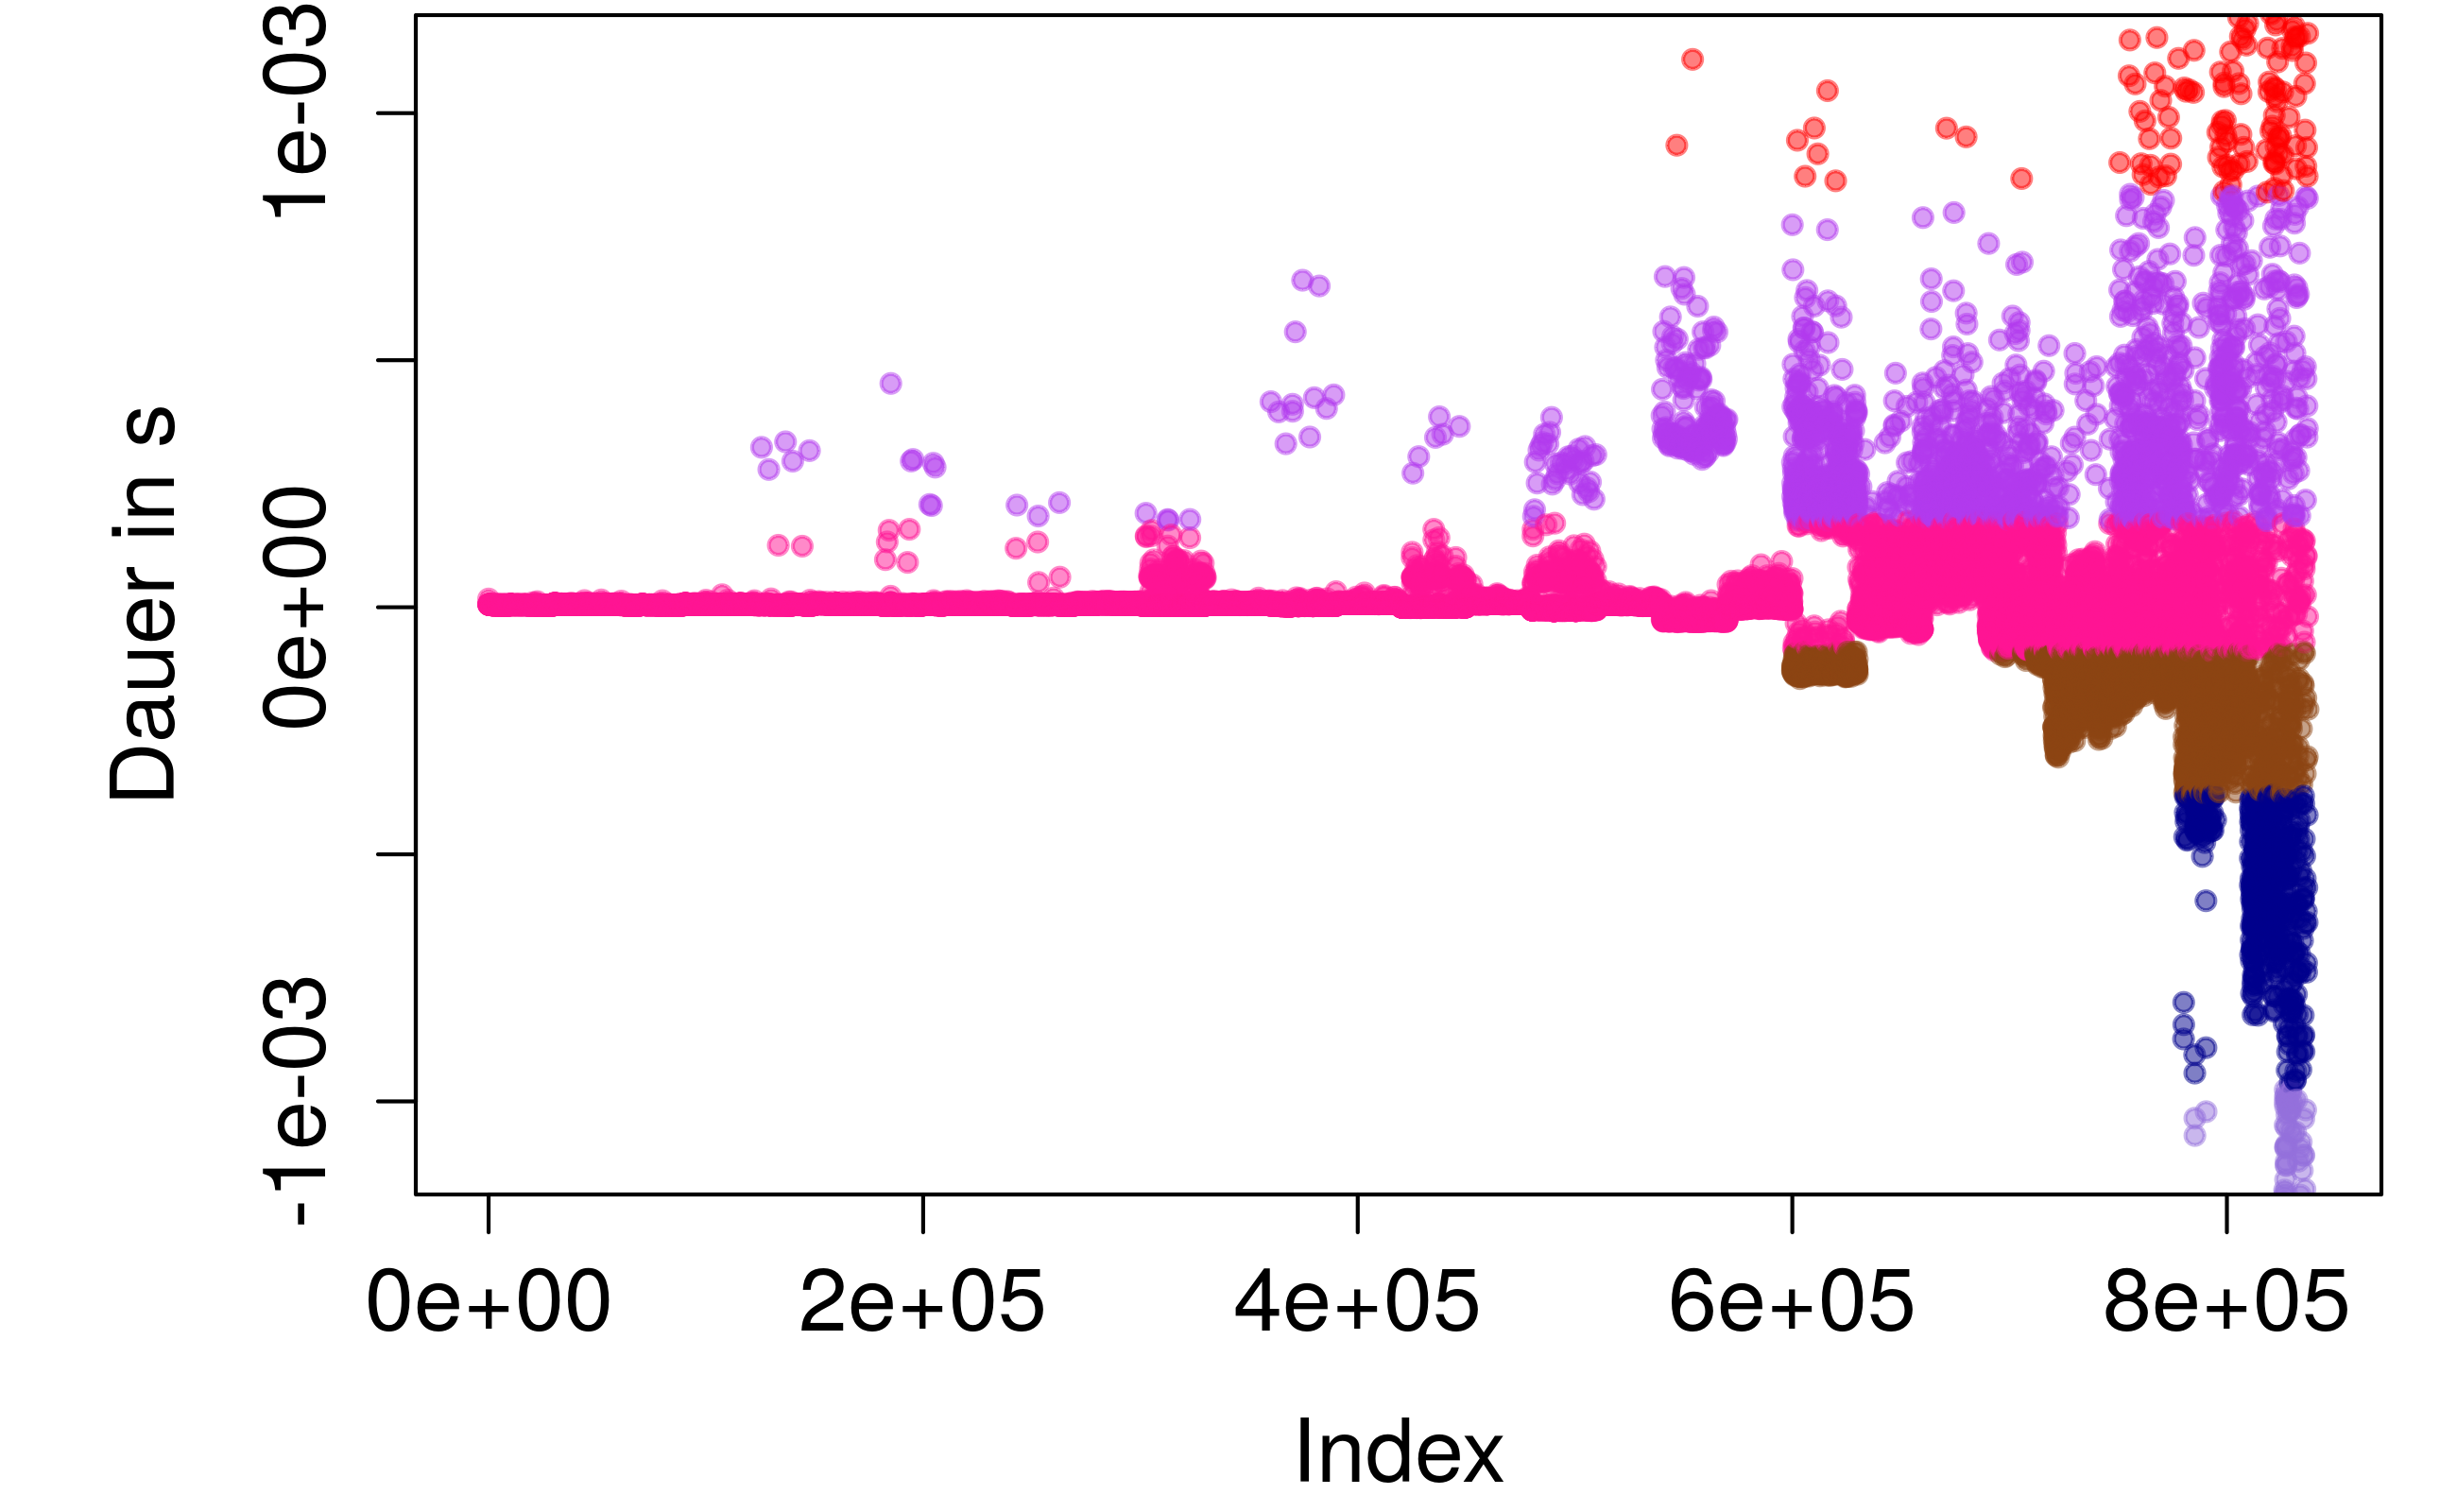
\includegraphics[width=.55\textwidth]{src/linreg_error_clustering_seq_all.png}
%		%}
%		\begin{tikzpicture}[spy using outlines={circle,black}] %,magnification=2.5,size=4.5cm, connect spies}]
%		\node {\pgfimage[interpolate=true,width=.53\textwidth]{src/linreg_error_clustering_seq_all.png}};
%		\draw (3.7,0.9) ellipse (0.8 and 0.8);
%		%\spy on (3.5,0.5) in node [left]; % at (14,1.25);
%		\end{tikzpicture}
%		\\
%		%\hfill
%		\subfloat[Random access pattern]{
%			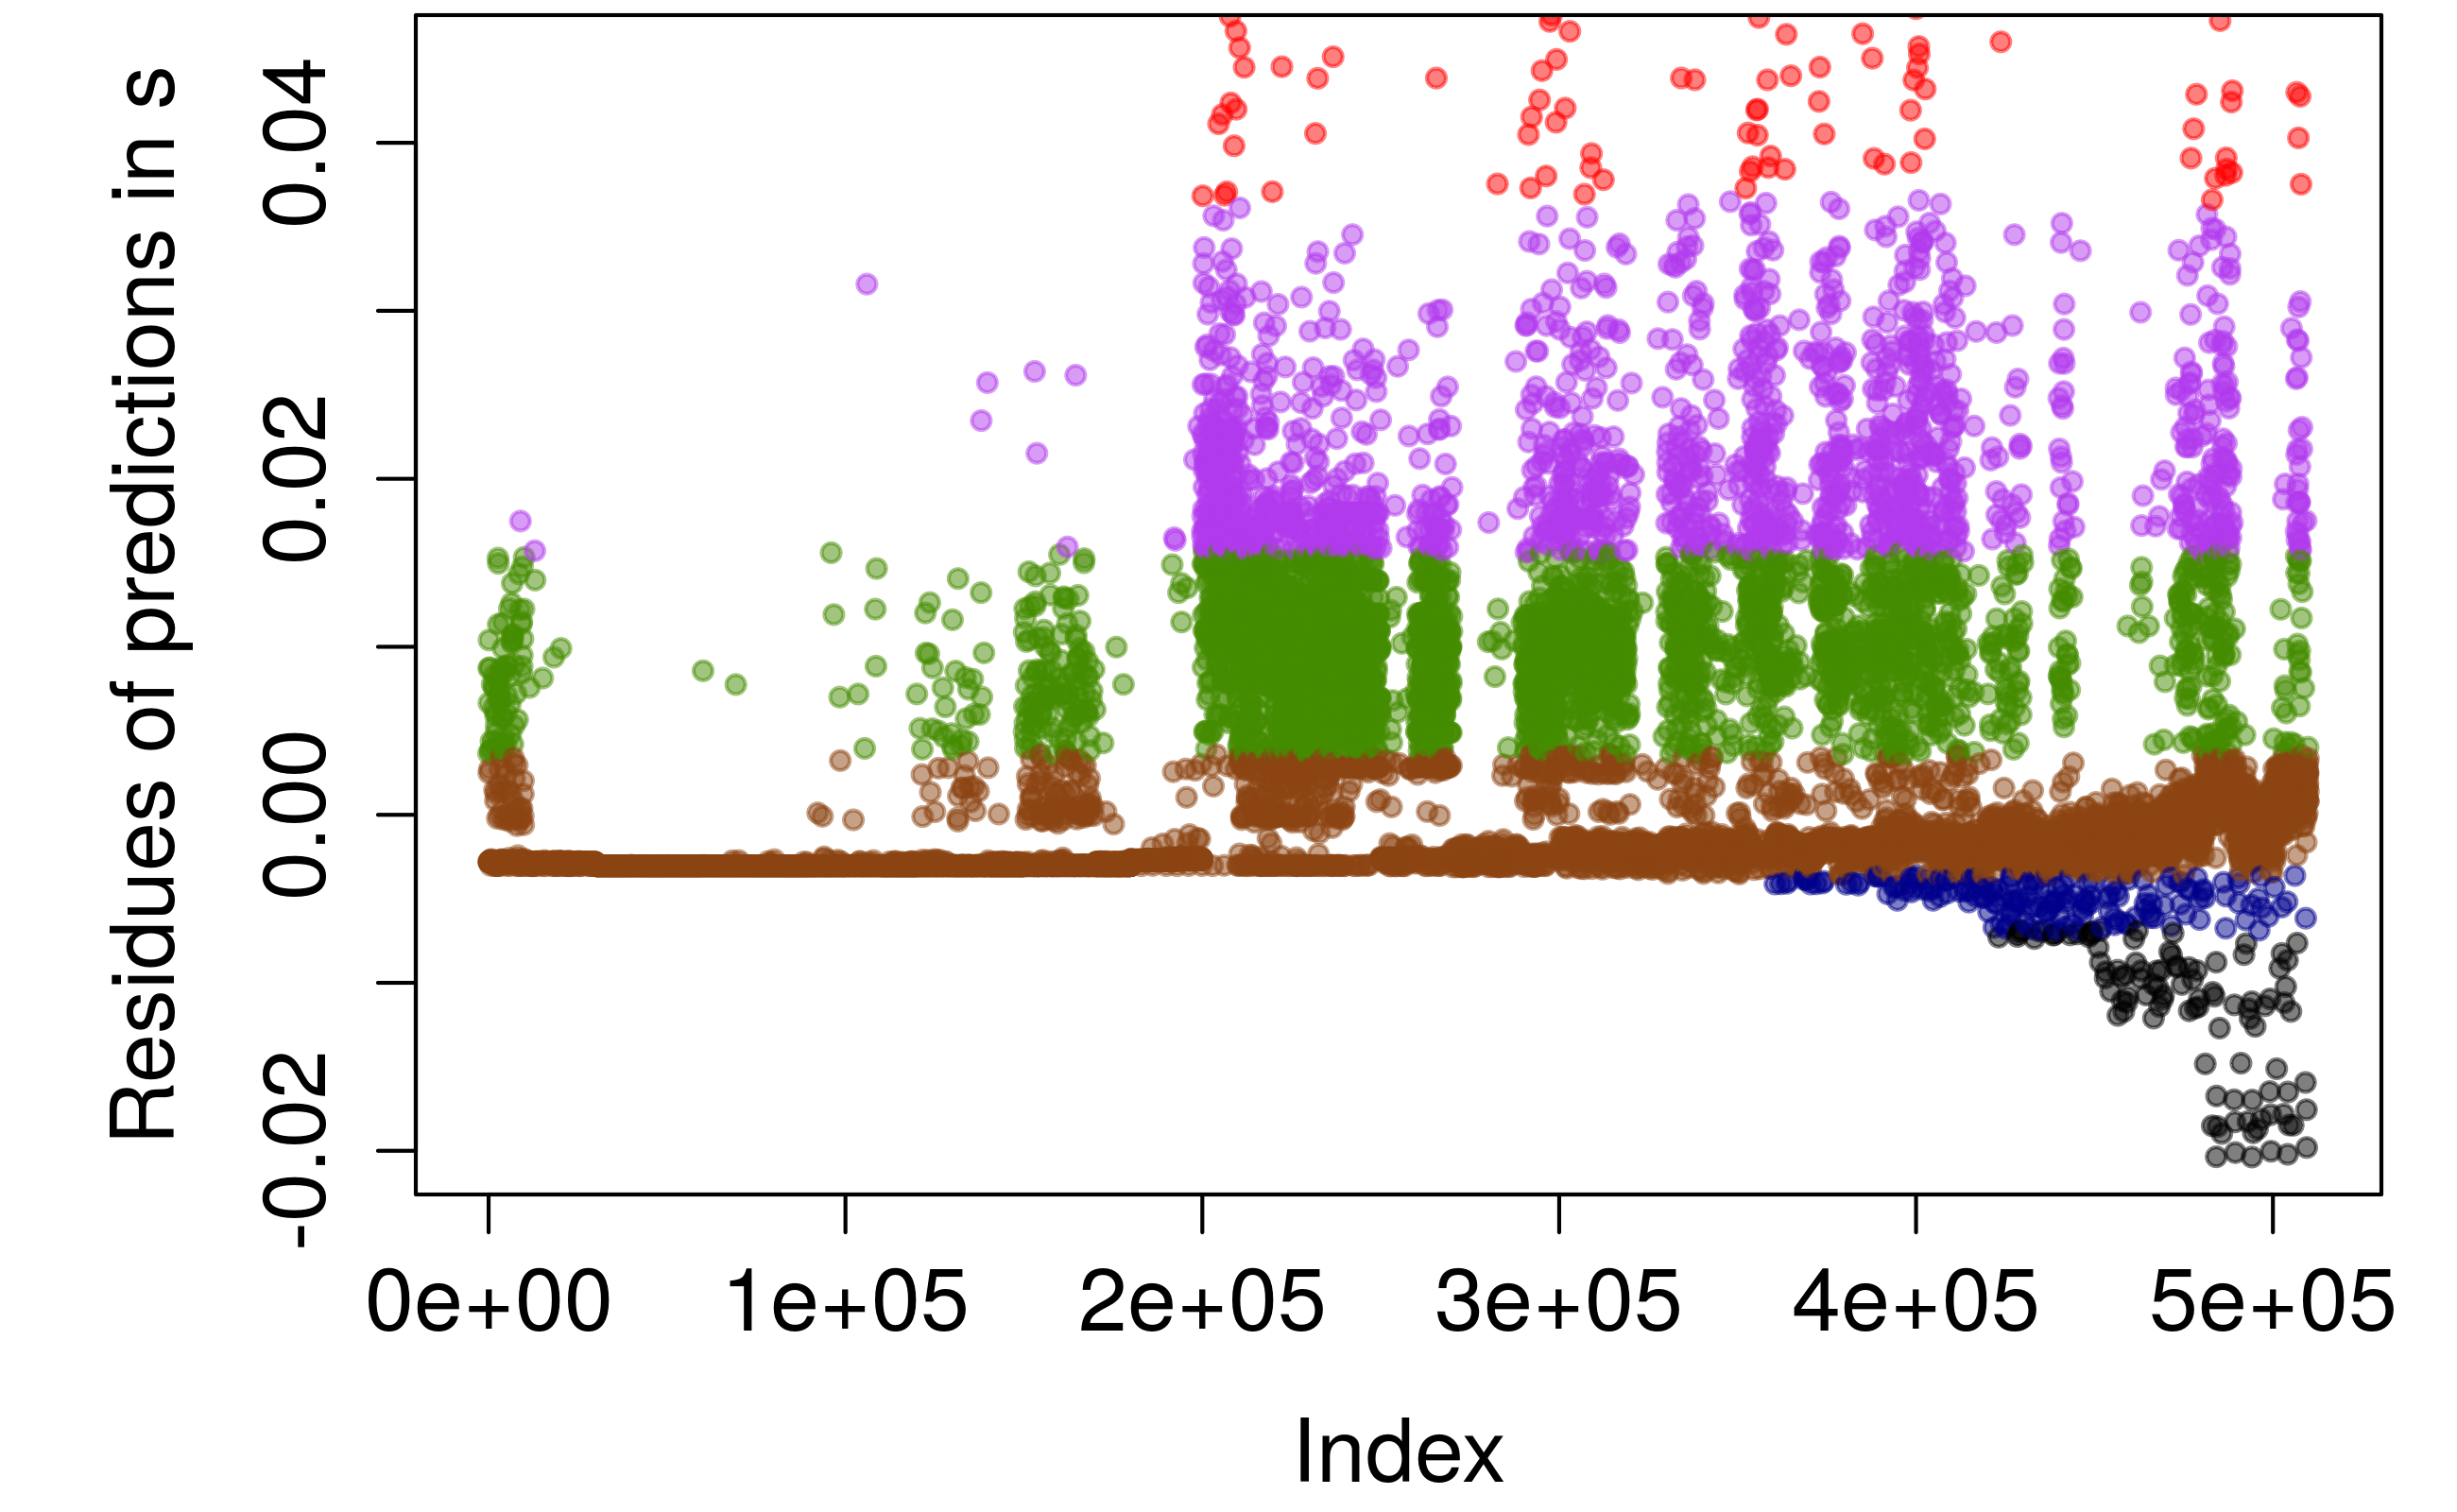
\includegraphics[width=.53\textwidth]{src/linreg_error_clustering_rnd_all.png}
%		}	
%		\caption{Residues from the linear regression model clustered into error classes. In the highlighted section the differen- tiation of measurements with varying I/O-paths can be seen.}
%		\label{error_classes}
%	\end{figure} 
	
		\begin{figure}
			%\flushleft
			\captionsetup[subfigure]{margin={-0.4cm,0cm}}
			\subfloat[Sequential access pattern]{
				%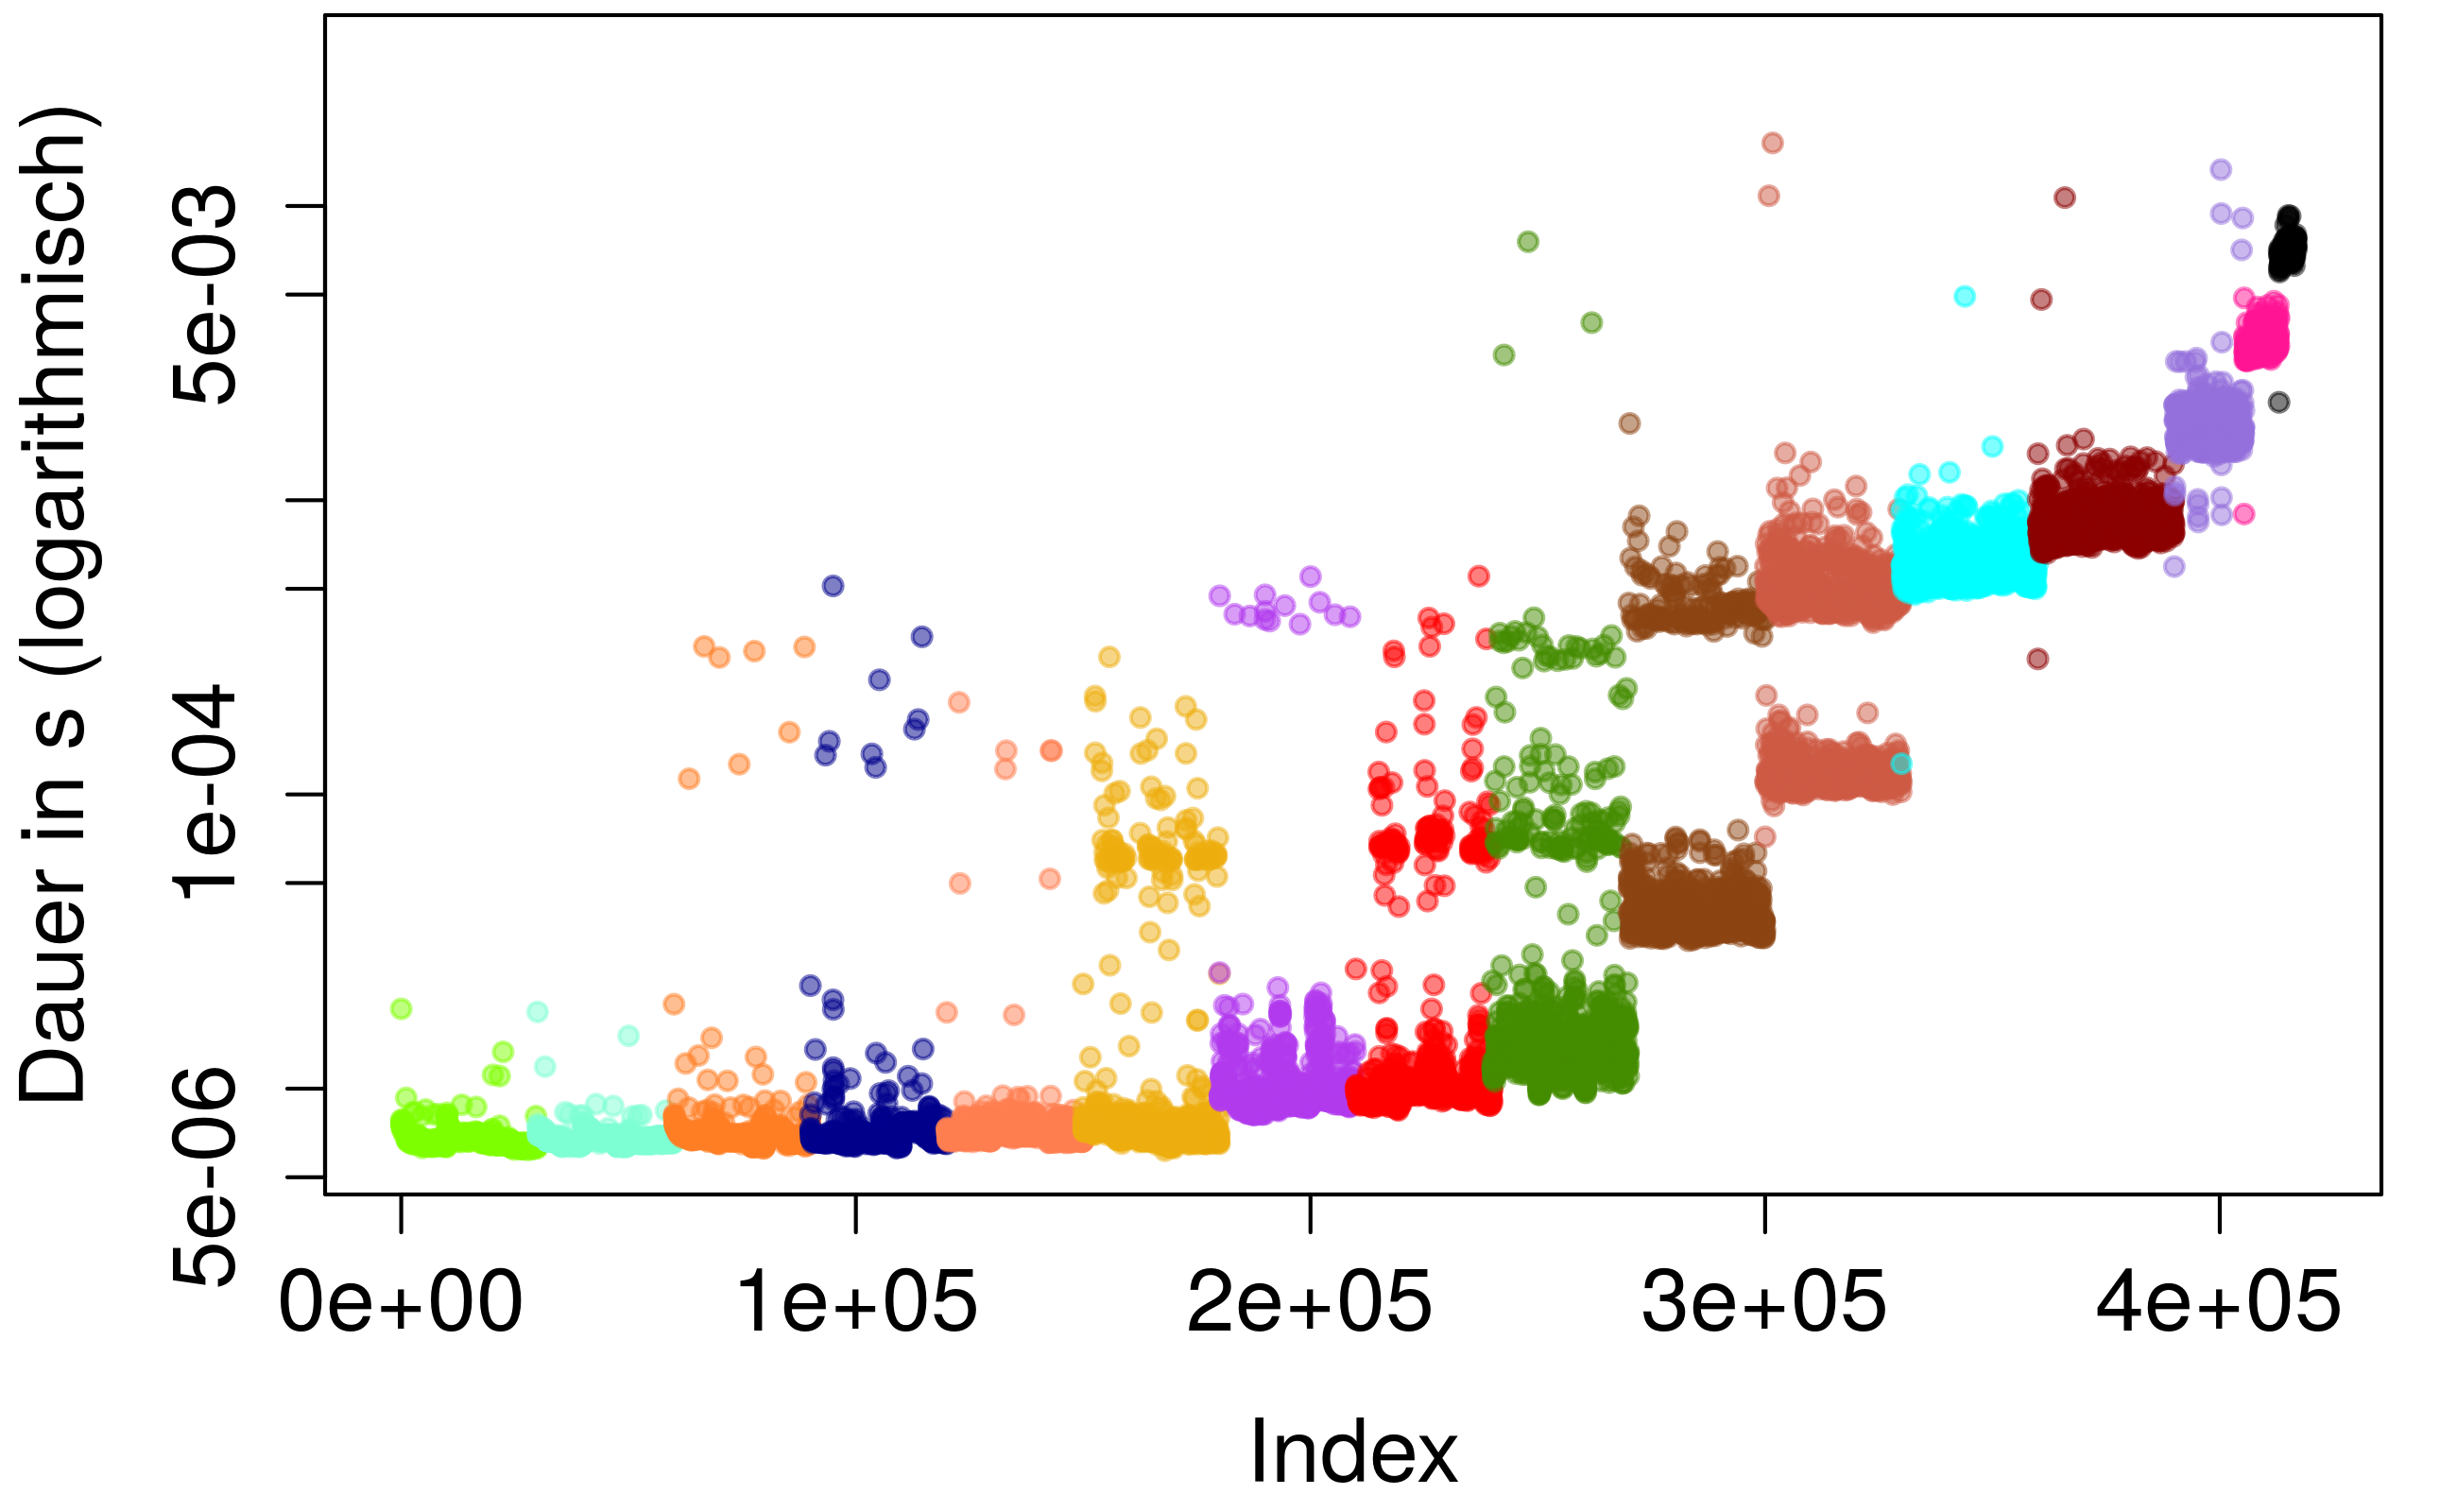
\includegraphics[width=.55\textwidth]{src/plot_SizeSorted_log_read_seq.png}
				\begin{tikzpicture}[spy using outlines={circle,black,magnification=2.2,size=4cm, connect spies}]
				\node {\pgfimage[interpolate=true,width=.53\textwidth]{src/linreg_error_clustering_seq_all.png}};
				%\draw (3.5,0.5) ellipse (1 and 1);
				\spy on (3.5,0.9) in node [left] at (14,1.25);
				\end{tikzpicture}
			}
			%\hfill
			\\
			\captionsetup[subfigure]{margin={-0.4cm,0cm}}
			\hspace*{-7.365cm}	
			%\vspace*{0.25cm}	
			\subfloat[Random access pattern]{
				%\hspace*{-5cm}
				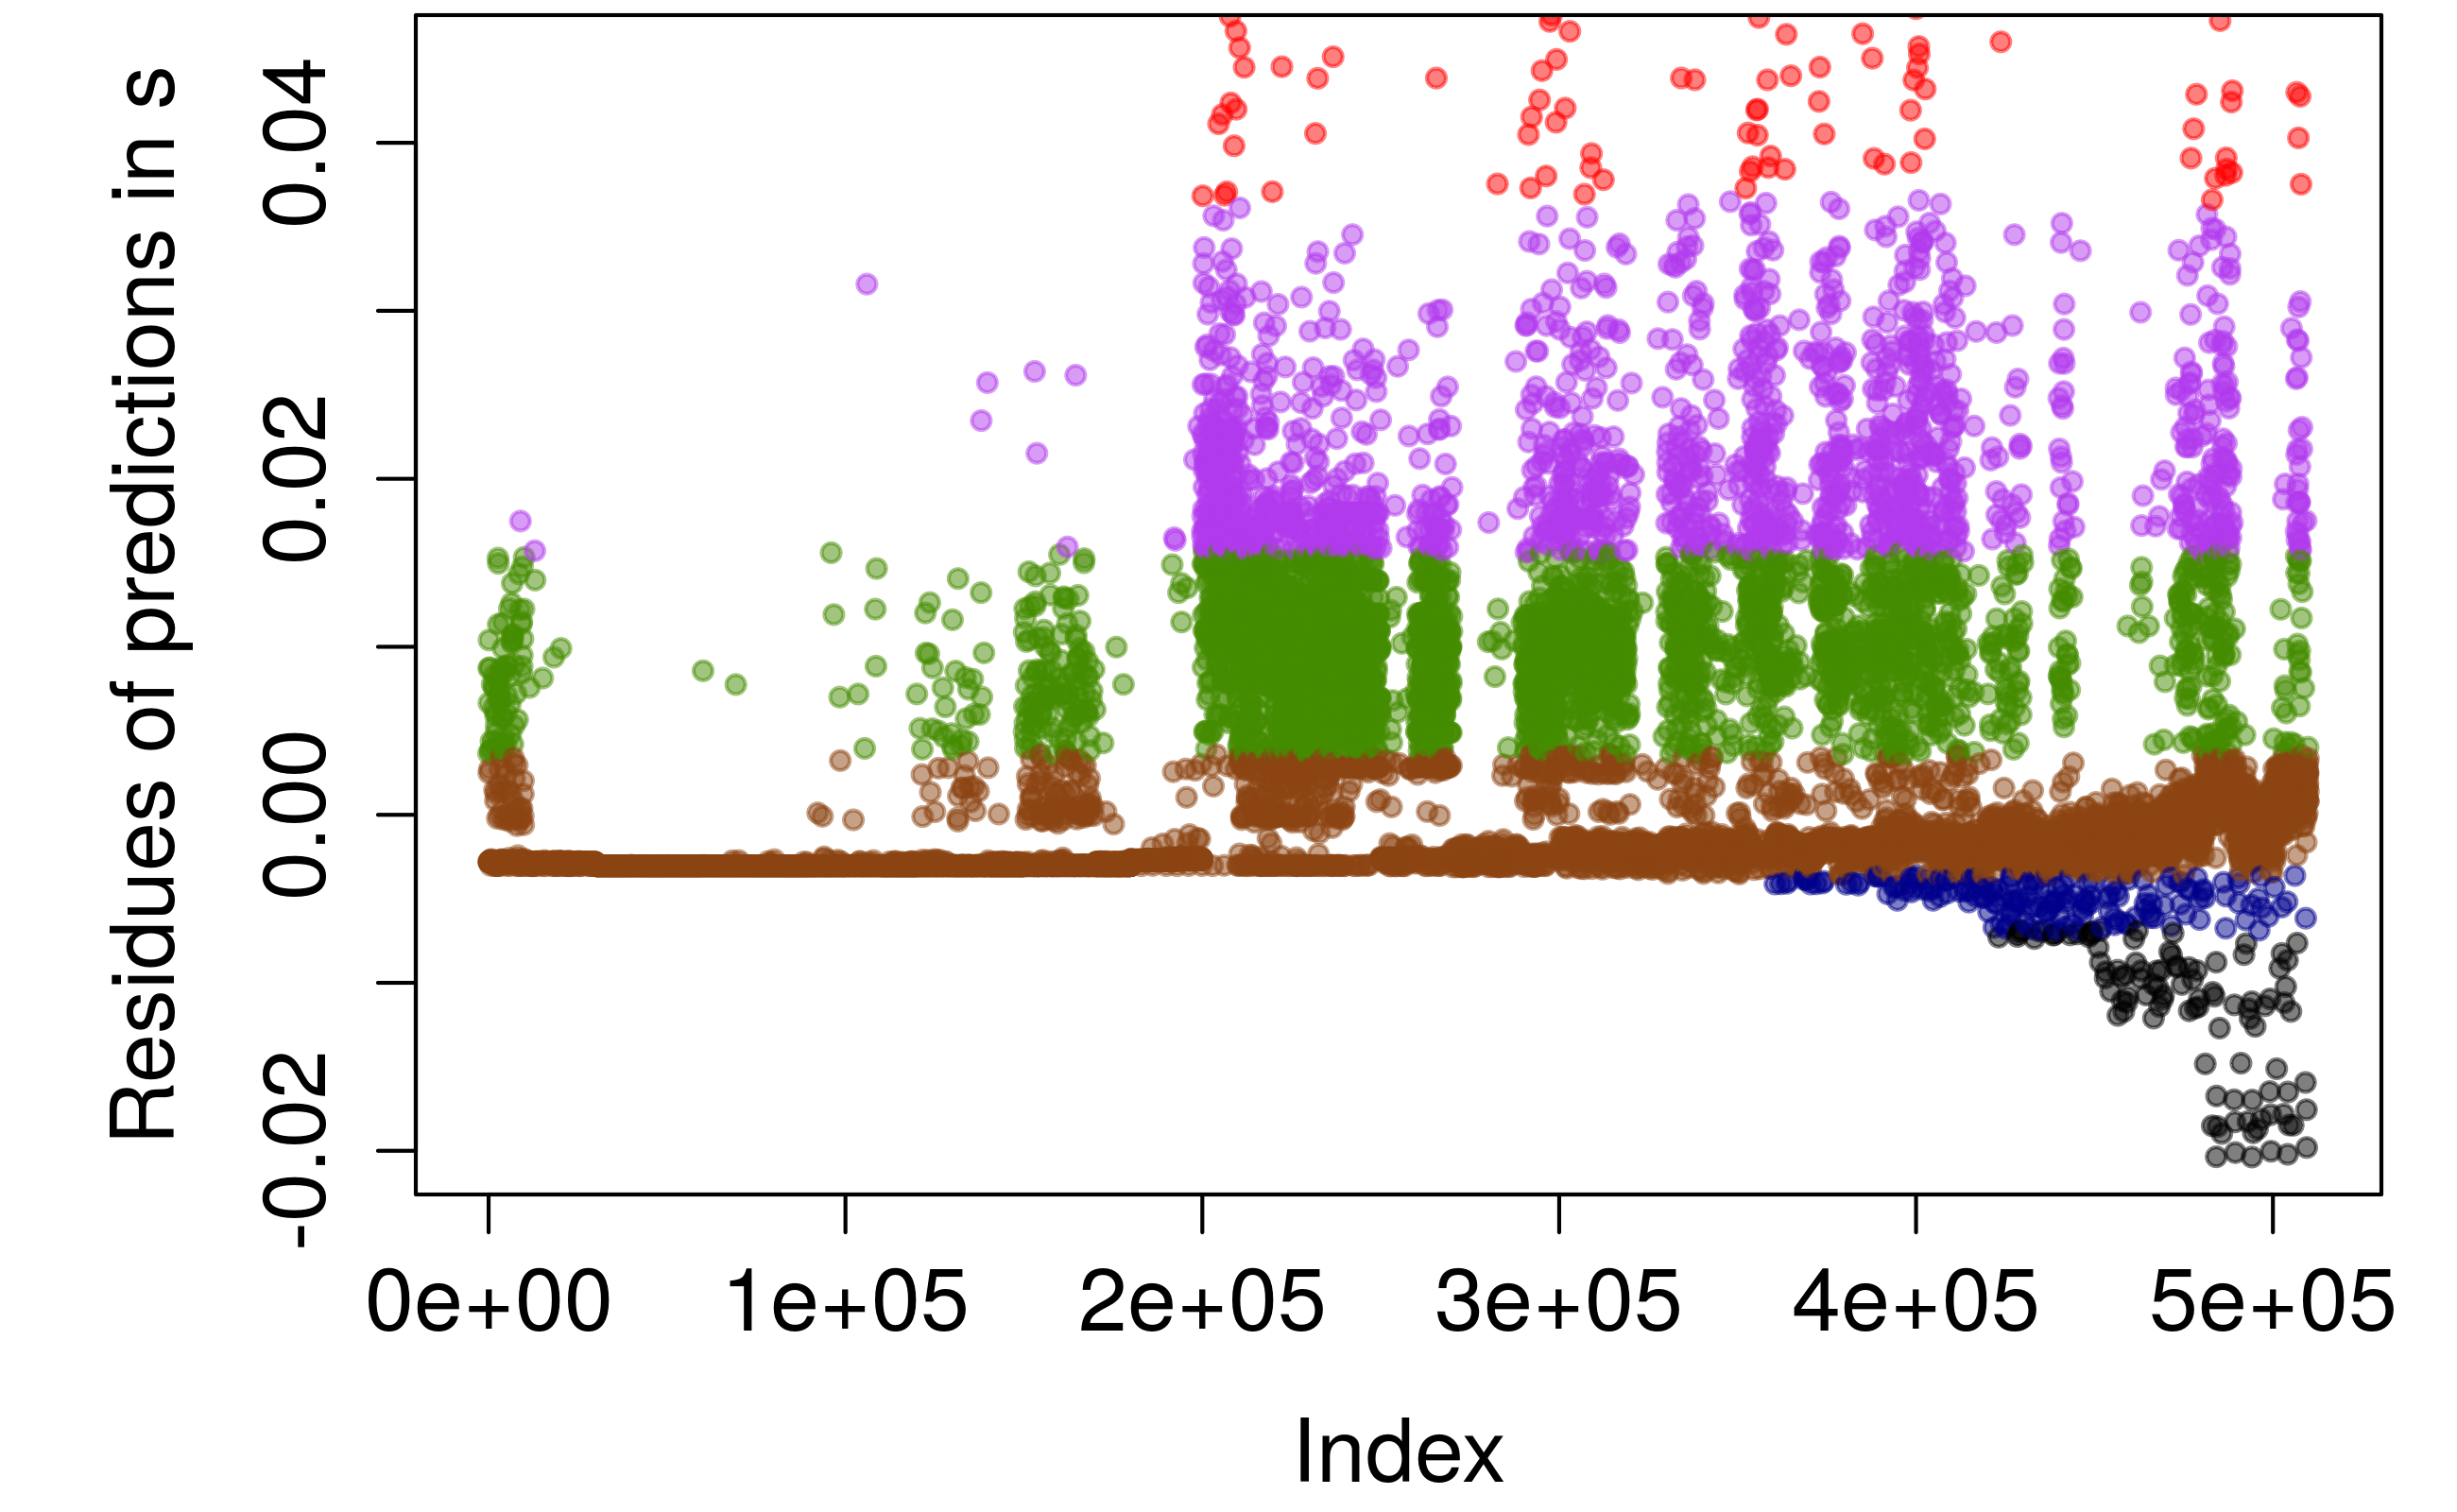
\includegraphics[width=.53\textwidth]{src/linreg_error_clustering_rnd_all.png}
			}
			\vspace*{-0.1cm}
			\caption{Residues from the linear regression model clustered into error classes. In the highlighted section the differen- tiation of measurements with varying I/O-paths can be seen.}
			\label{error_classes}
		\end{figure} 

%\begin{figure}
%	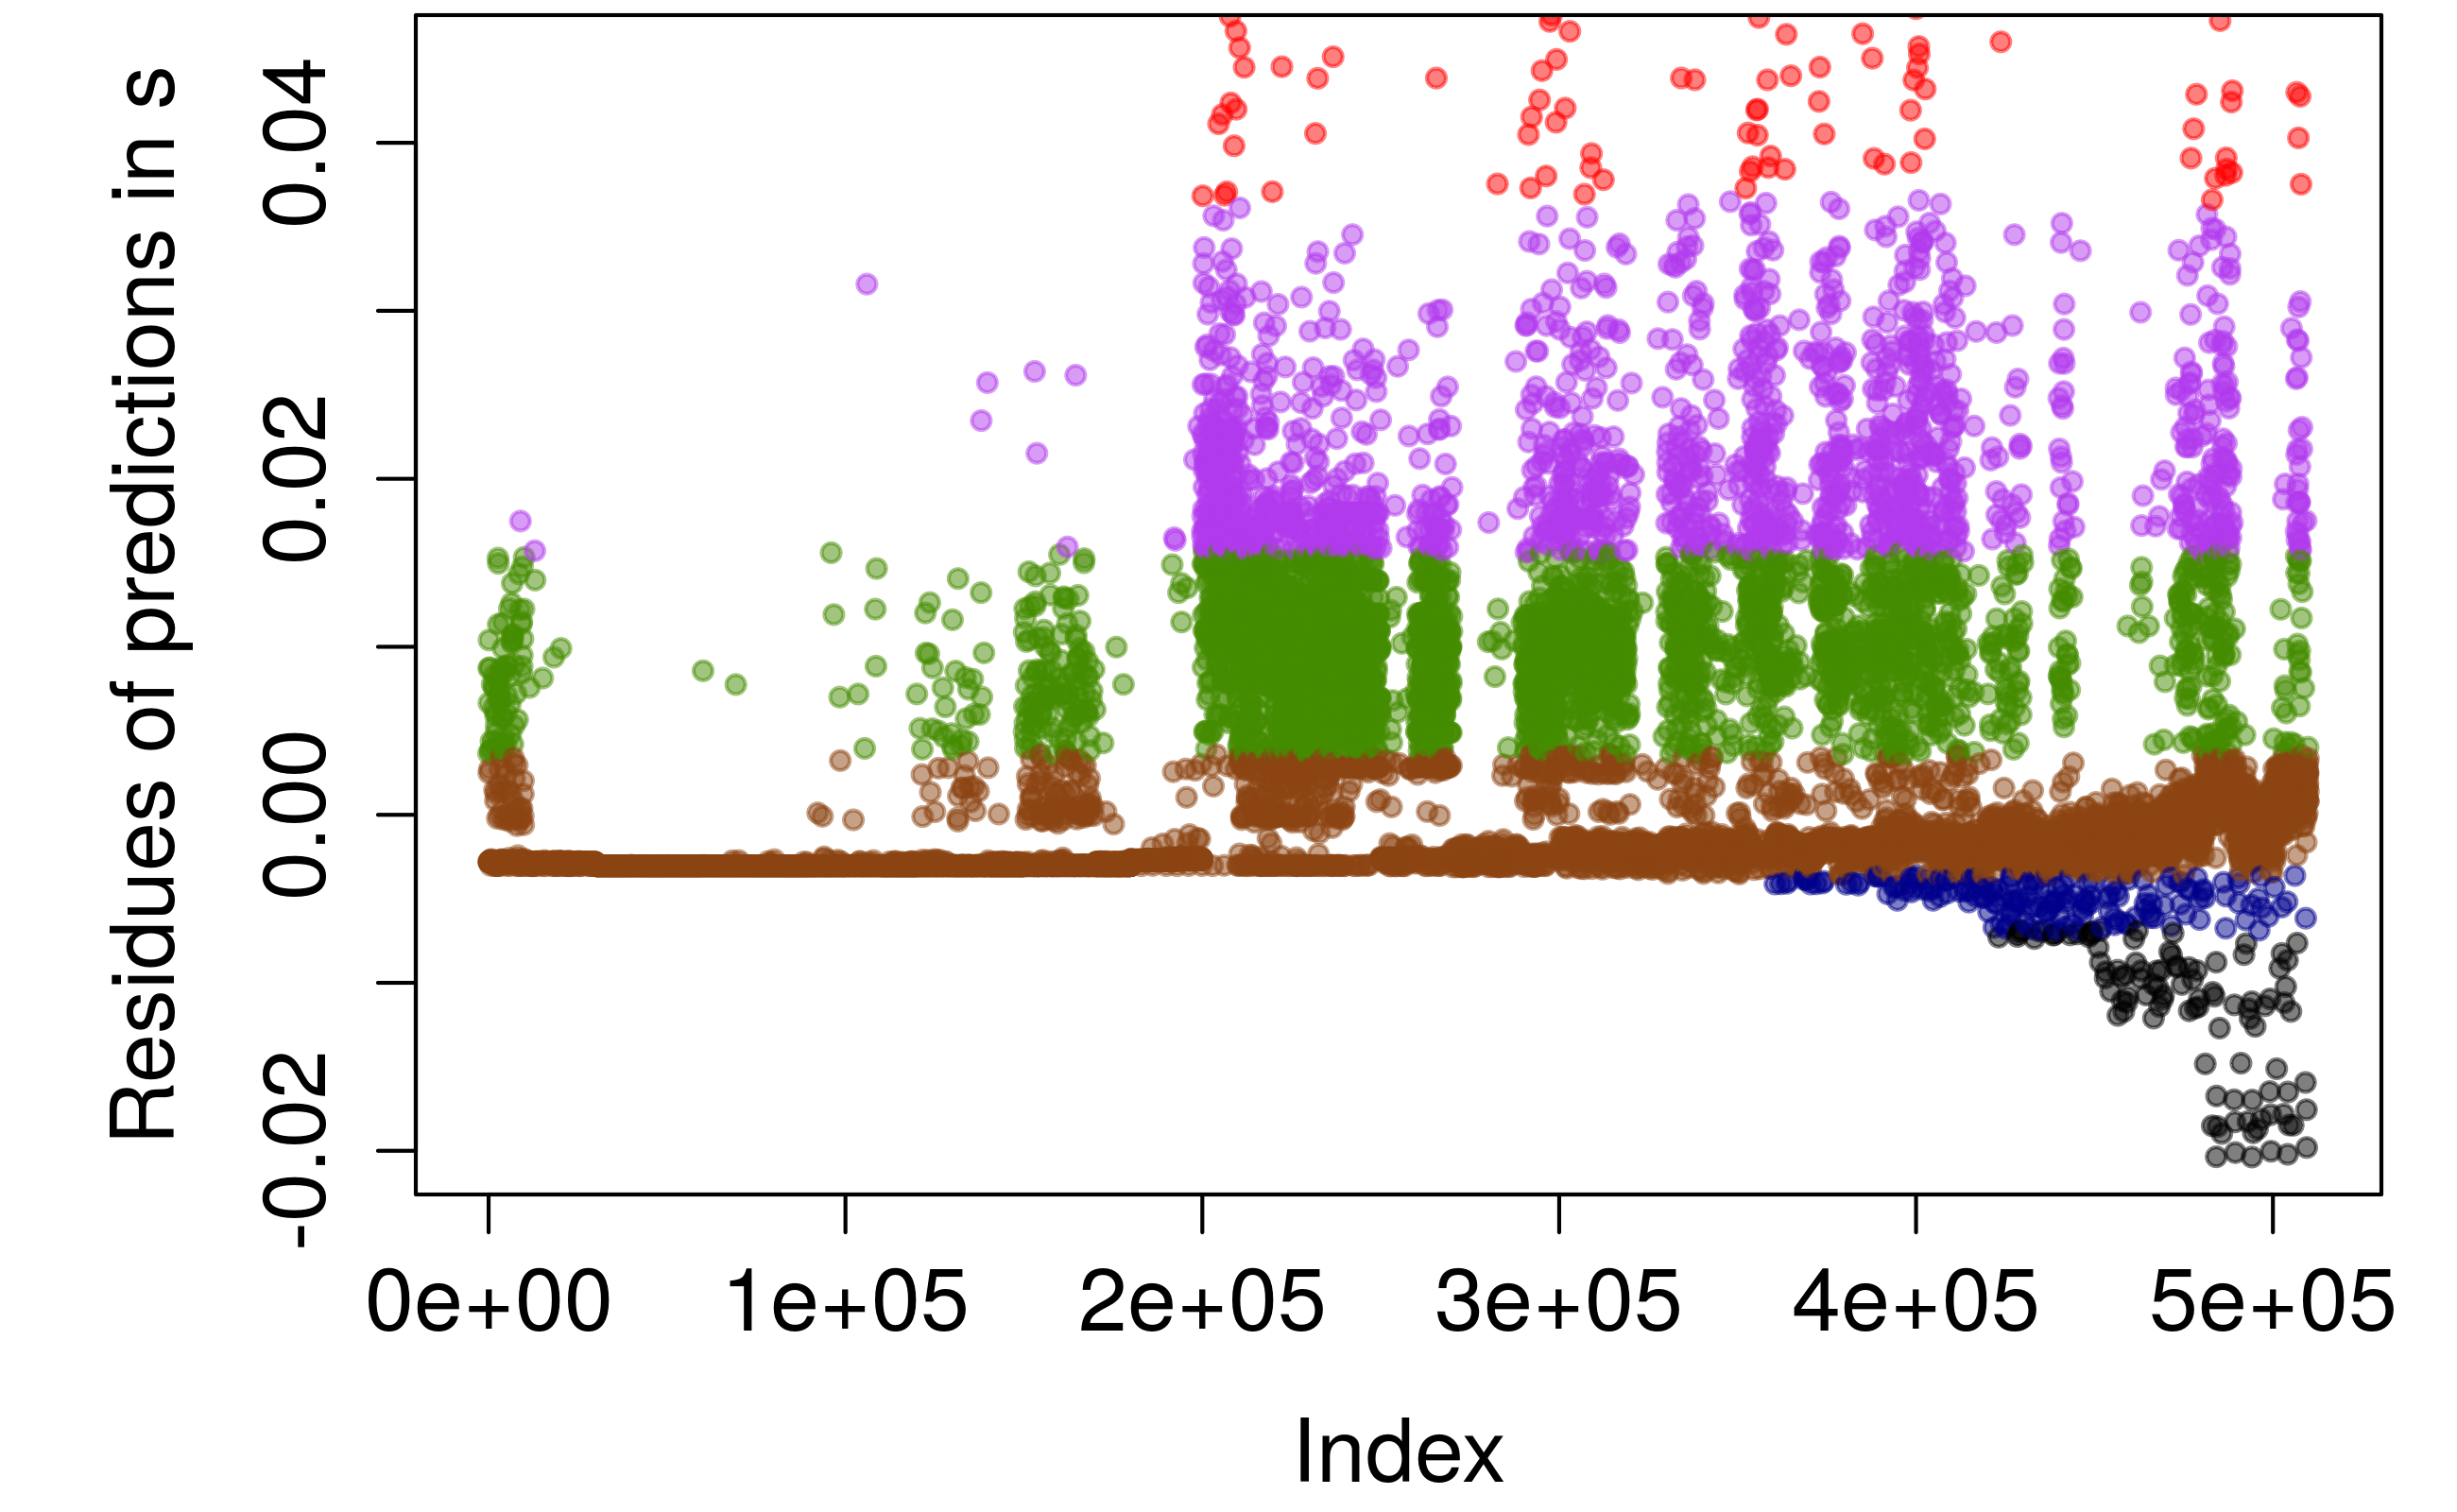
\includegraphics[width=0.7\linewidth]{src/linreg_error_clustering_rnd_all.png}
%	\vspace*{-0.5cm}
%	\caption{The clustering into error classes on the residues of the model with linear regression.}
%	\label{error_classes}
%\end{figure}

\end{block}

\end{column} % End of the 3 column

\begin{column}{\sepwid}\end{column} % Empty spacer column

\begin{column}{\onecolwid} % The 4 column

\begin{block}{Results}
	
	From the residues of our models (see table \ref{residues}) it became clear that access times shouldn't be modelled linearly.
	Furthermore the exploitation of time dependencies of the storage system has been found to be difficult.
	As our hypothesis predicted \textbf{it is essential to use knowledge about I/O-paths for precise predictions of access times}.
	The error classes allow the ANN to decrease the error significantly.
	In figure \ref{preds} the benefit of error classes as input can be seen:
	The second ANN is often able to classify file accesses correctly in respect to their I/O-path.
	
	\begin{table}
		\scriptsize
		\vspace{0.2cm}
		\begin{tabular}{l|r|r|r|r}%
			&  \multicolumn{2}{|c}{MAE (s)}&  \multicolumn{2}{|c}{MSPE (\%)}\\ \hline
			%\toprule
			Modell & seq. access & rnd. access & seq. access & rnd. access\\ \hline
			%\midrule
			Linear regression & $7.6\cdot 10^-5$ & $4.76\cdot 10^-3$ & 59 & 14185  \\
			ANN & $6.0\cdot 10^-5$ & $3.13\cdot 10^-3$ & 22 & 530 \\
			ANN + time dependencies & $5.7\cdot 10^-5$ & $3.05\cdot 10^-3$ & 22 & 619\\
			ANN + error classes & $2.0\cdot 10^-5$ & $1.03\cdot 10^-3$ & 14 & 119\\
			%\bottomrule
		\end{tabular}
		\caption{Mean absolut errors and mean square percentage errors of the models for two different file access patterns.}
		\label{residues}
	\end{table}
	
%		\begin{tabular}{|r|r|r|r|r|r|r|r|r|}\hline%
%			& \multicolumn{3}{|c|}{gemittelte Angaben} & \multicolumn{3}{|c|}{Angaben zu den Residuen} & \multicolumn{2}{r|}{zugeordnete Messungen} \\ \hline
%			Klasse & Durchsatz (B/s) & Größe (B) & Dauer (s) & Min (s) & Durchschnitt (s) & Max (s) & auf SEQ selbst & auf RND \\ \hline\hline
%			\csvreader[late after line=\\\hline]%
%			{CSV/error_class/seq_linreg_classes_on_rnd.csv}{tp=\tp,idx = \idx,rndcount=\rndcount,minerror=\minerror, meanerror = \meanerror, maxerror = \maxerror, seqcount = \seqcount, size = \size, duration = \duration}%
%			{\idx & \tp & \size & \duration & \minerror & \meanerror & \maxerror & \seqcount & \rndcount}%
%		\end{tabular}
	
	\vspace*{-0.75cm}
	\begin{figure}
		\subfloat[ANN without error classes]{
			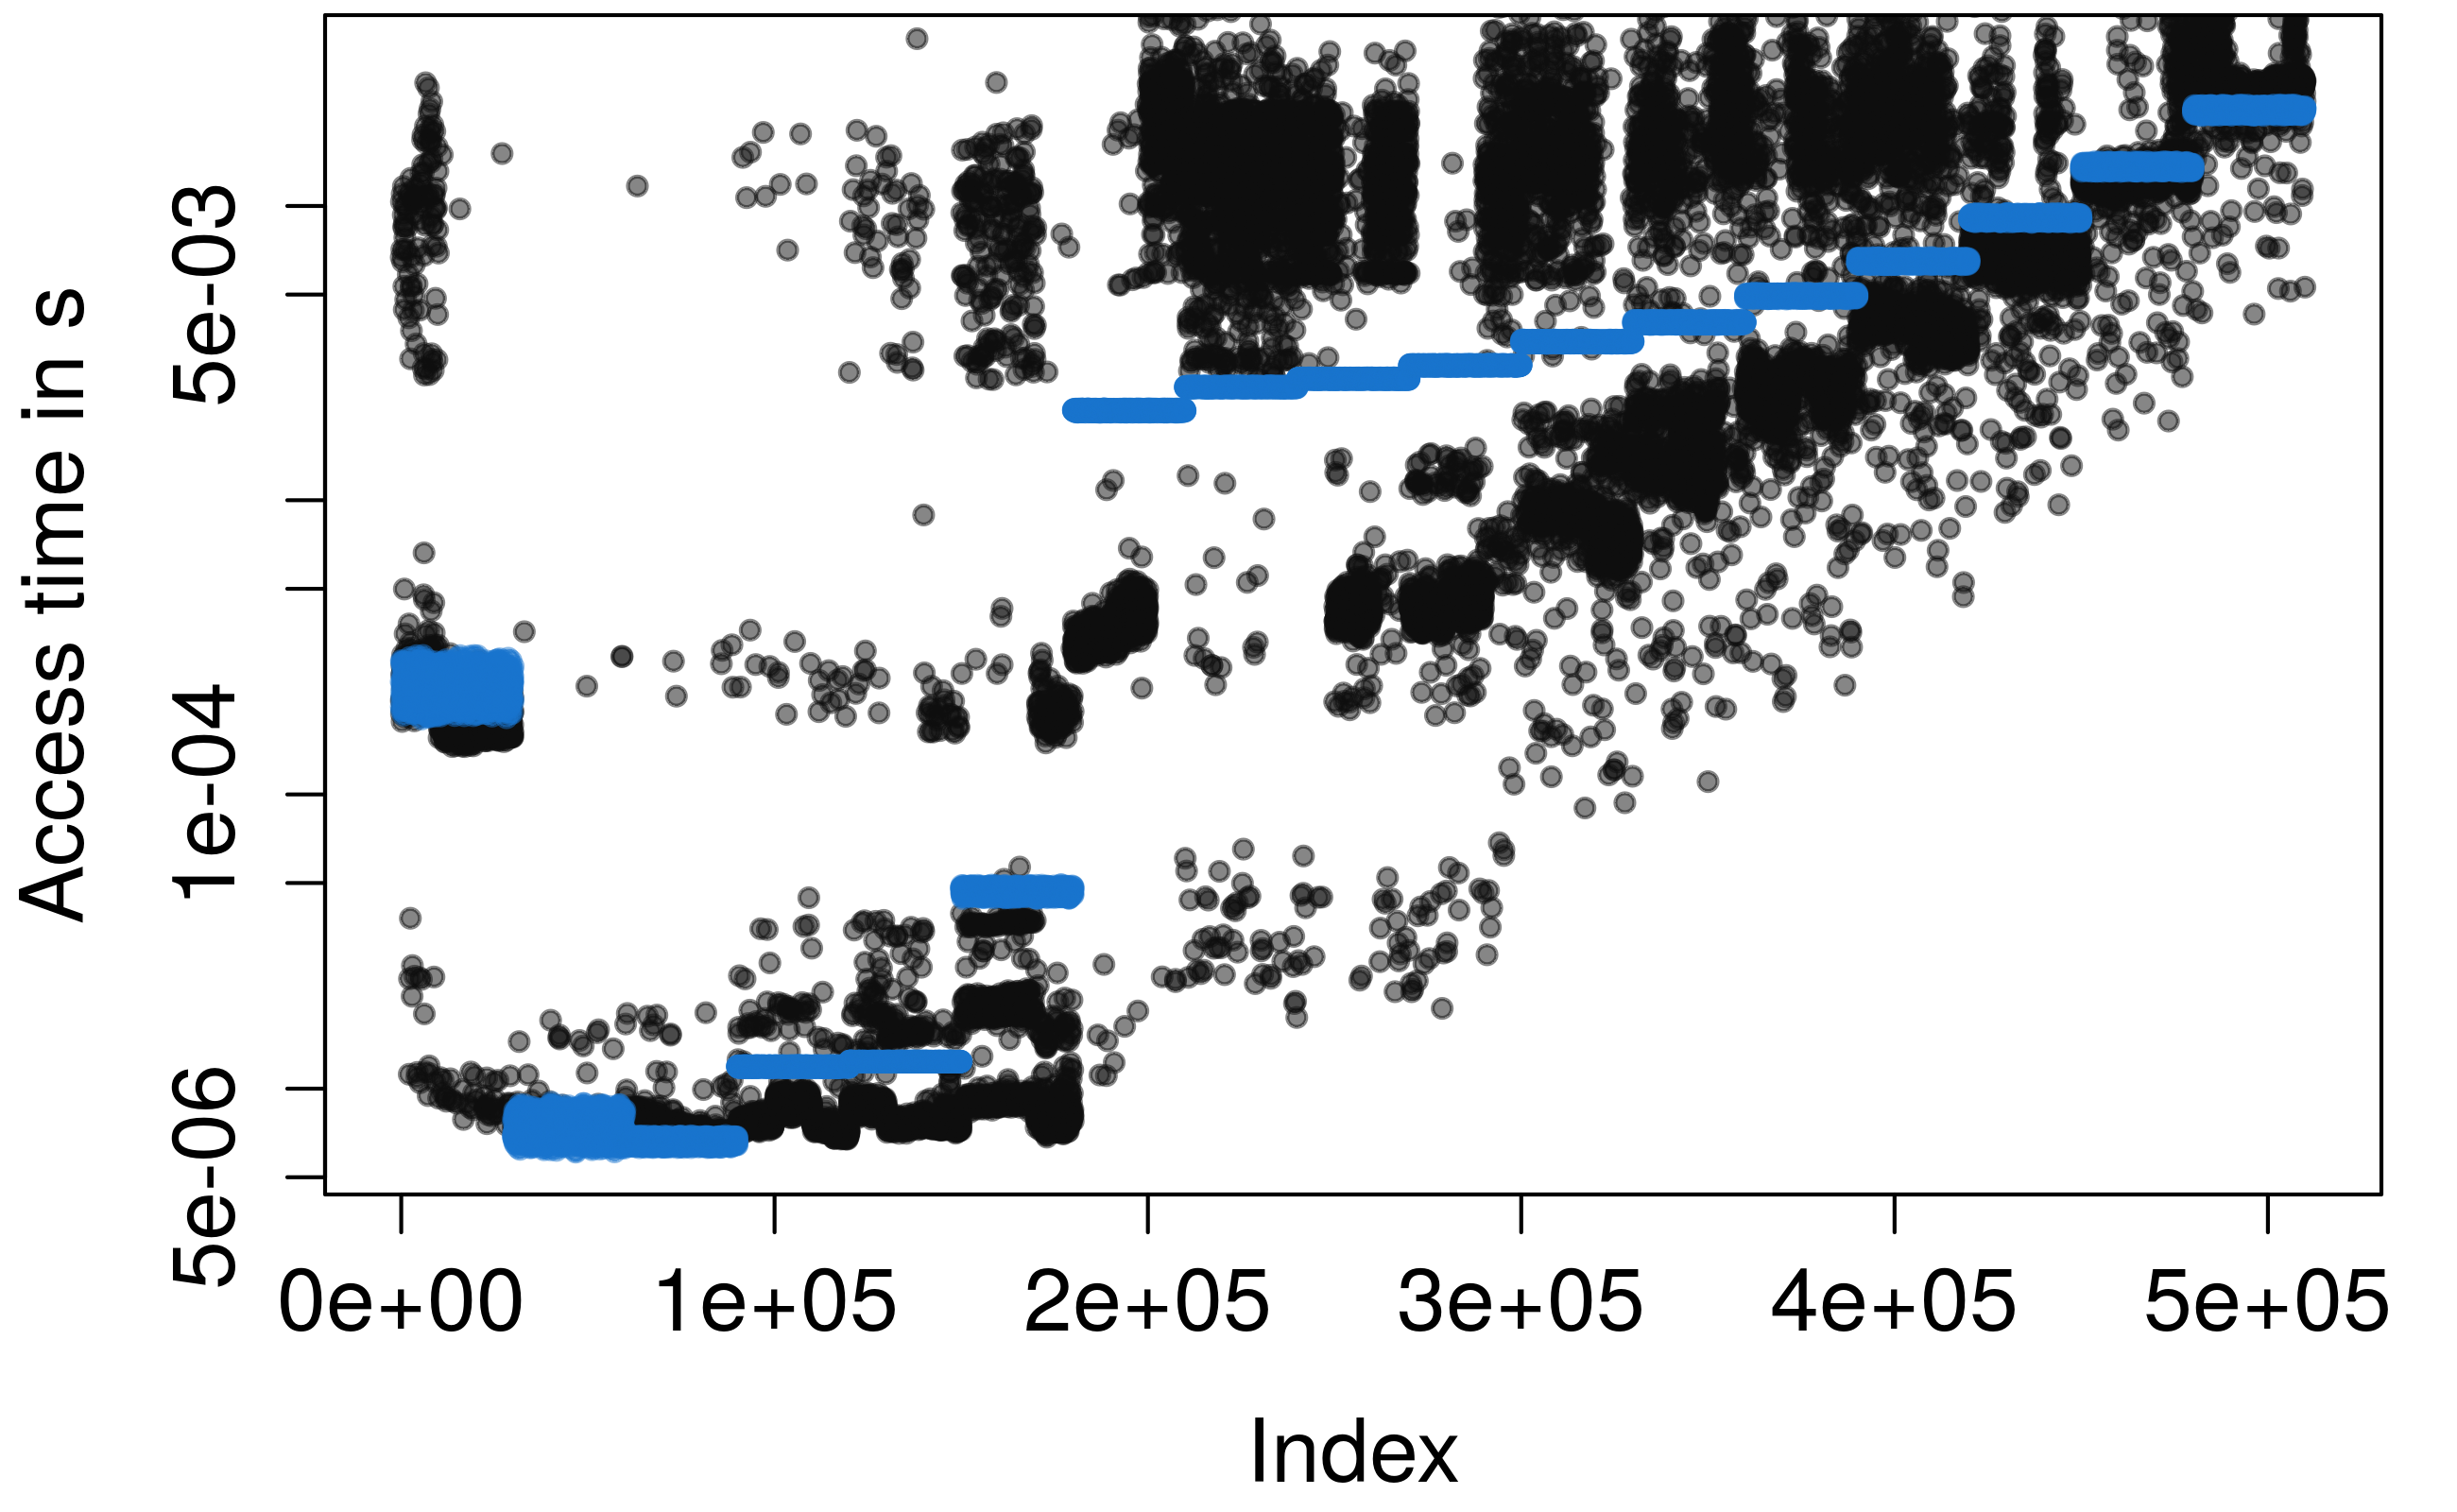
\includegraphics[width=.47\textwidth]{src/plot_onlyPred_tuple1_Duration_rnd.png}
		}
		\hfill		
		\subfloat[ANN with error classes]{
			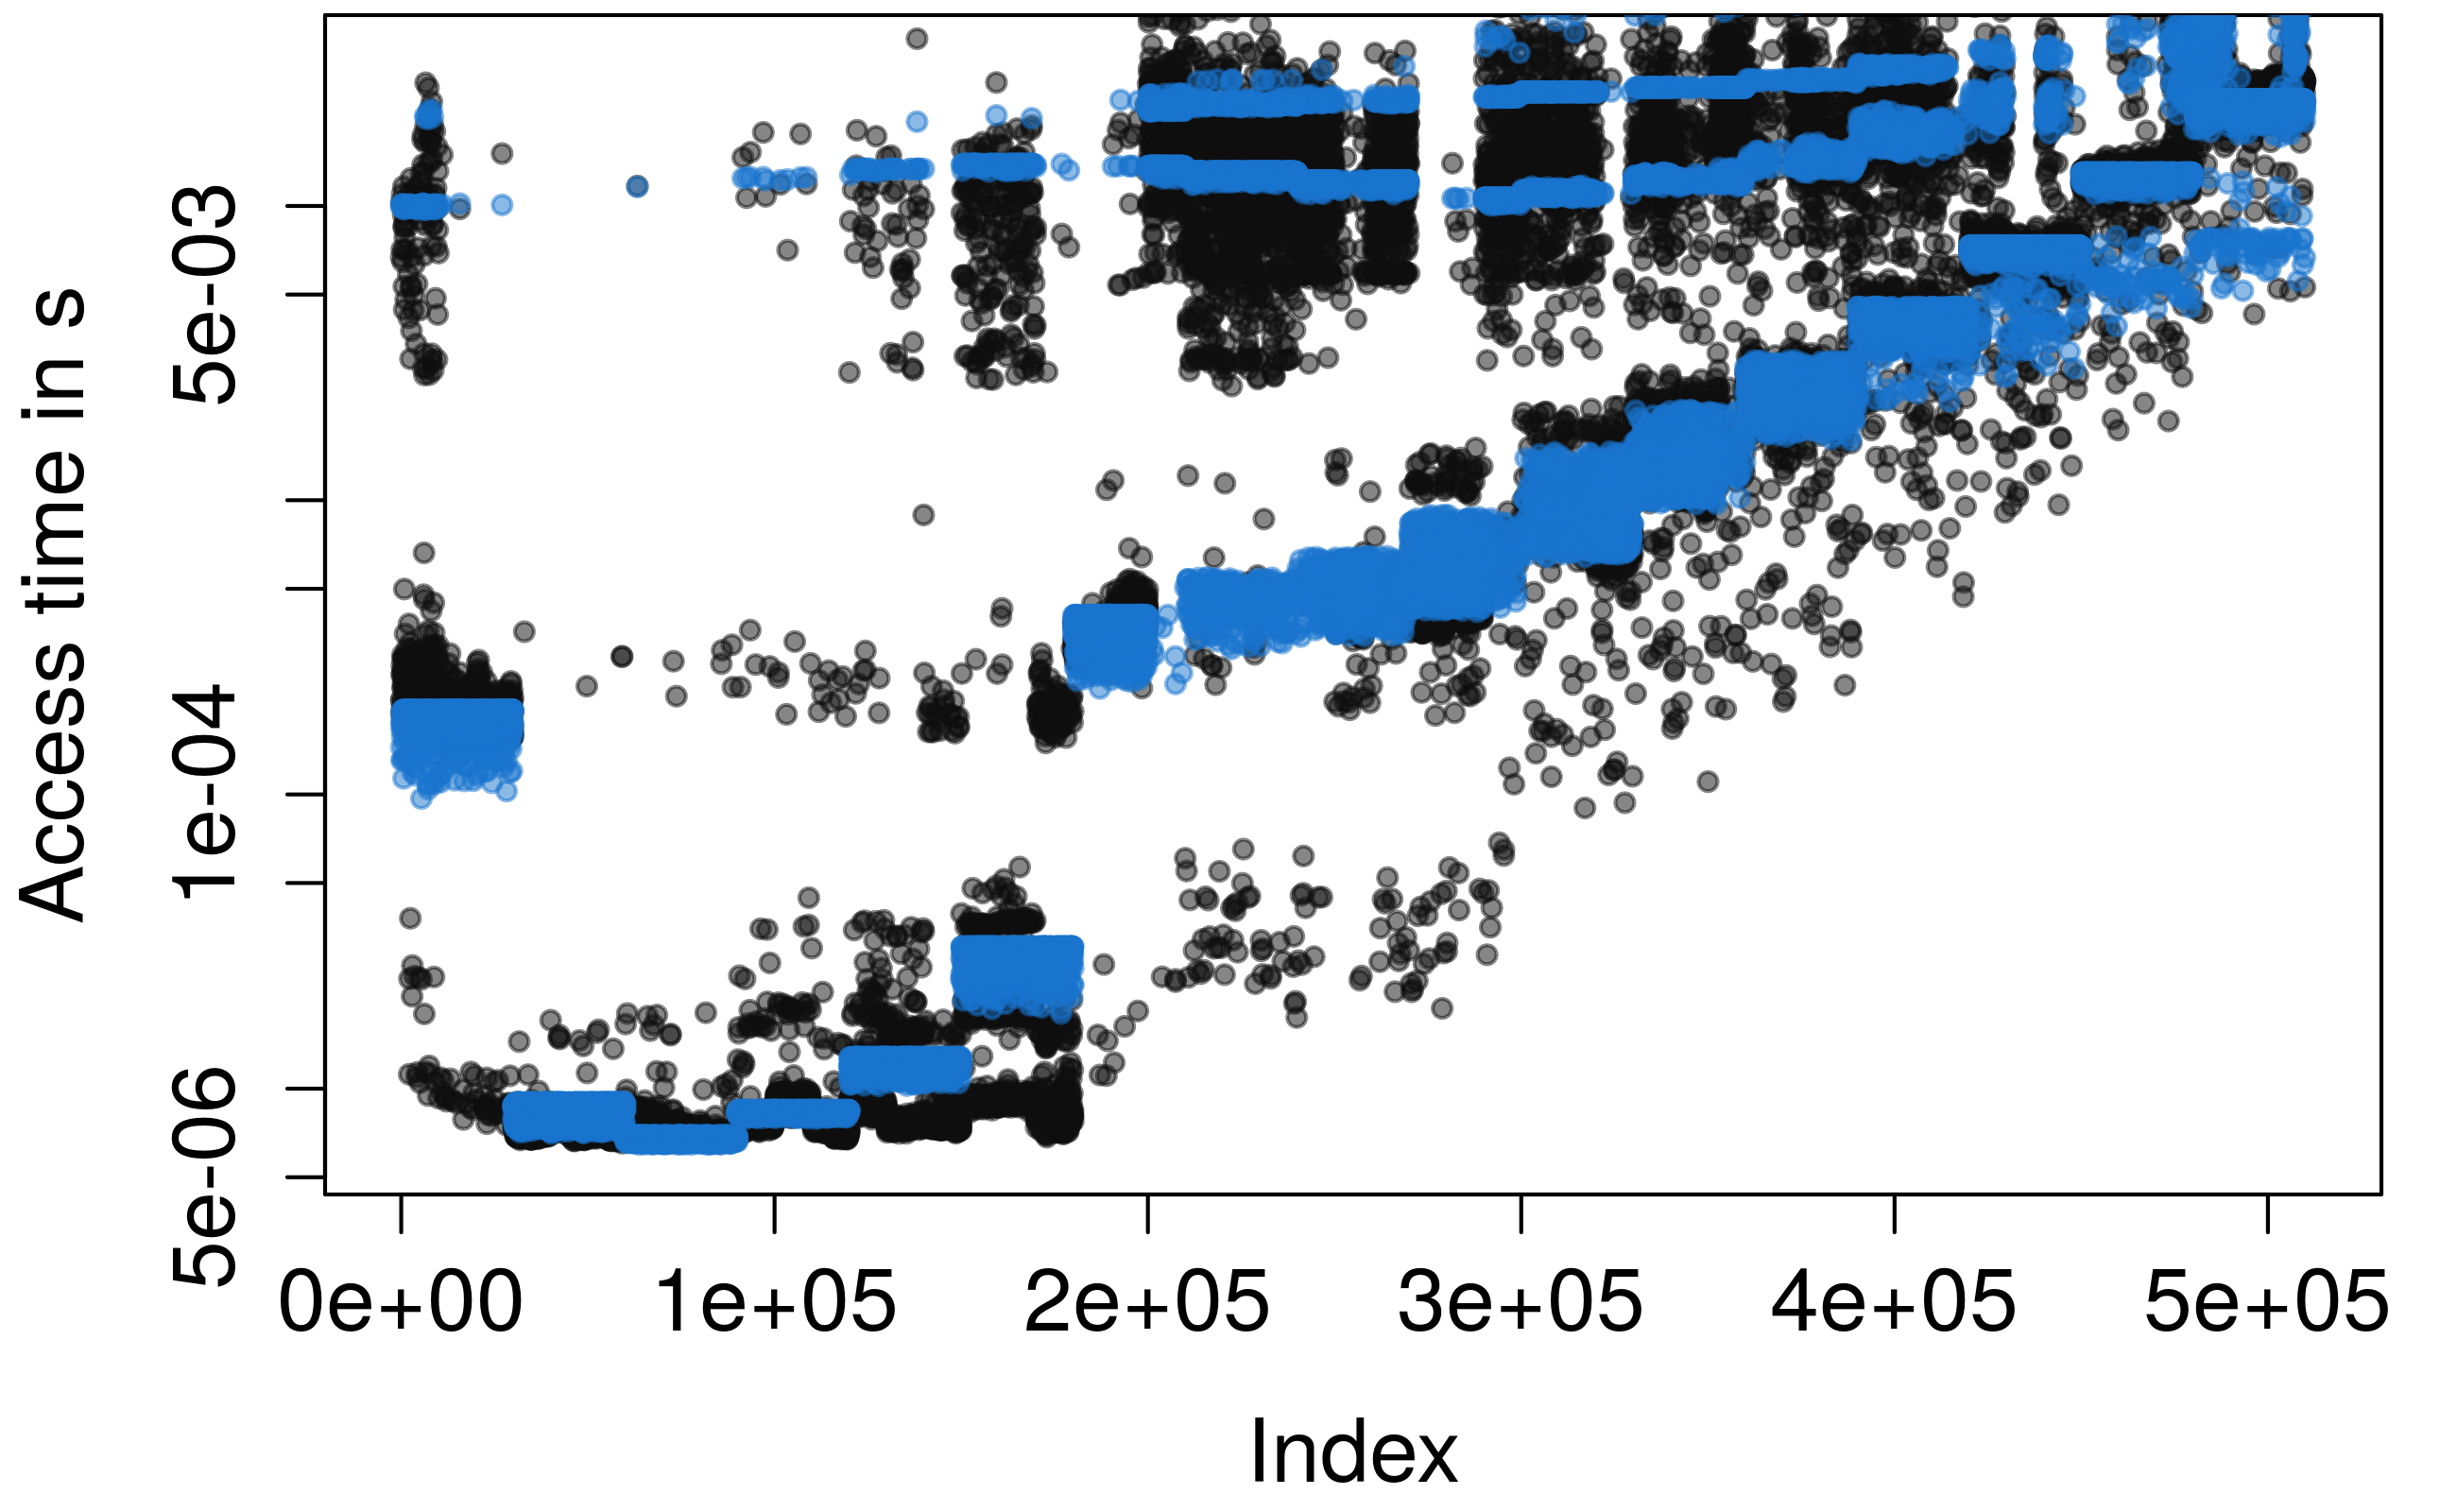
\includegraphics[width=.47\textwidth]{src/plot_onlyPred_tuple1_with_error_class_from_linreg_Duration_rnd.png}
		}	
		\caption{Measurements with random access pattern. Measured access times in black; predictions in blue.}
		\label{preds}
	\end{figure} 
%	
%	\begin{figure}
%		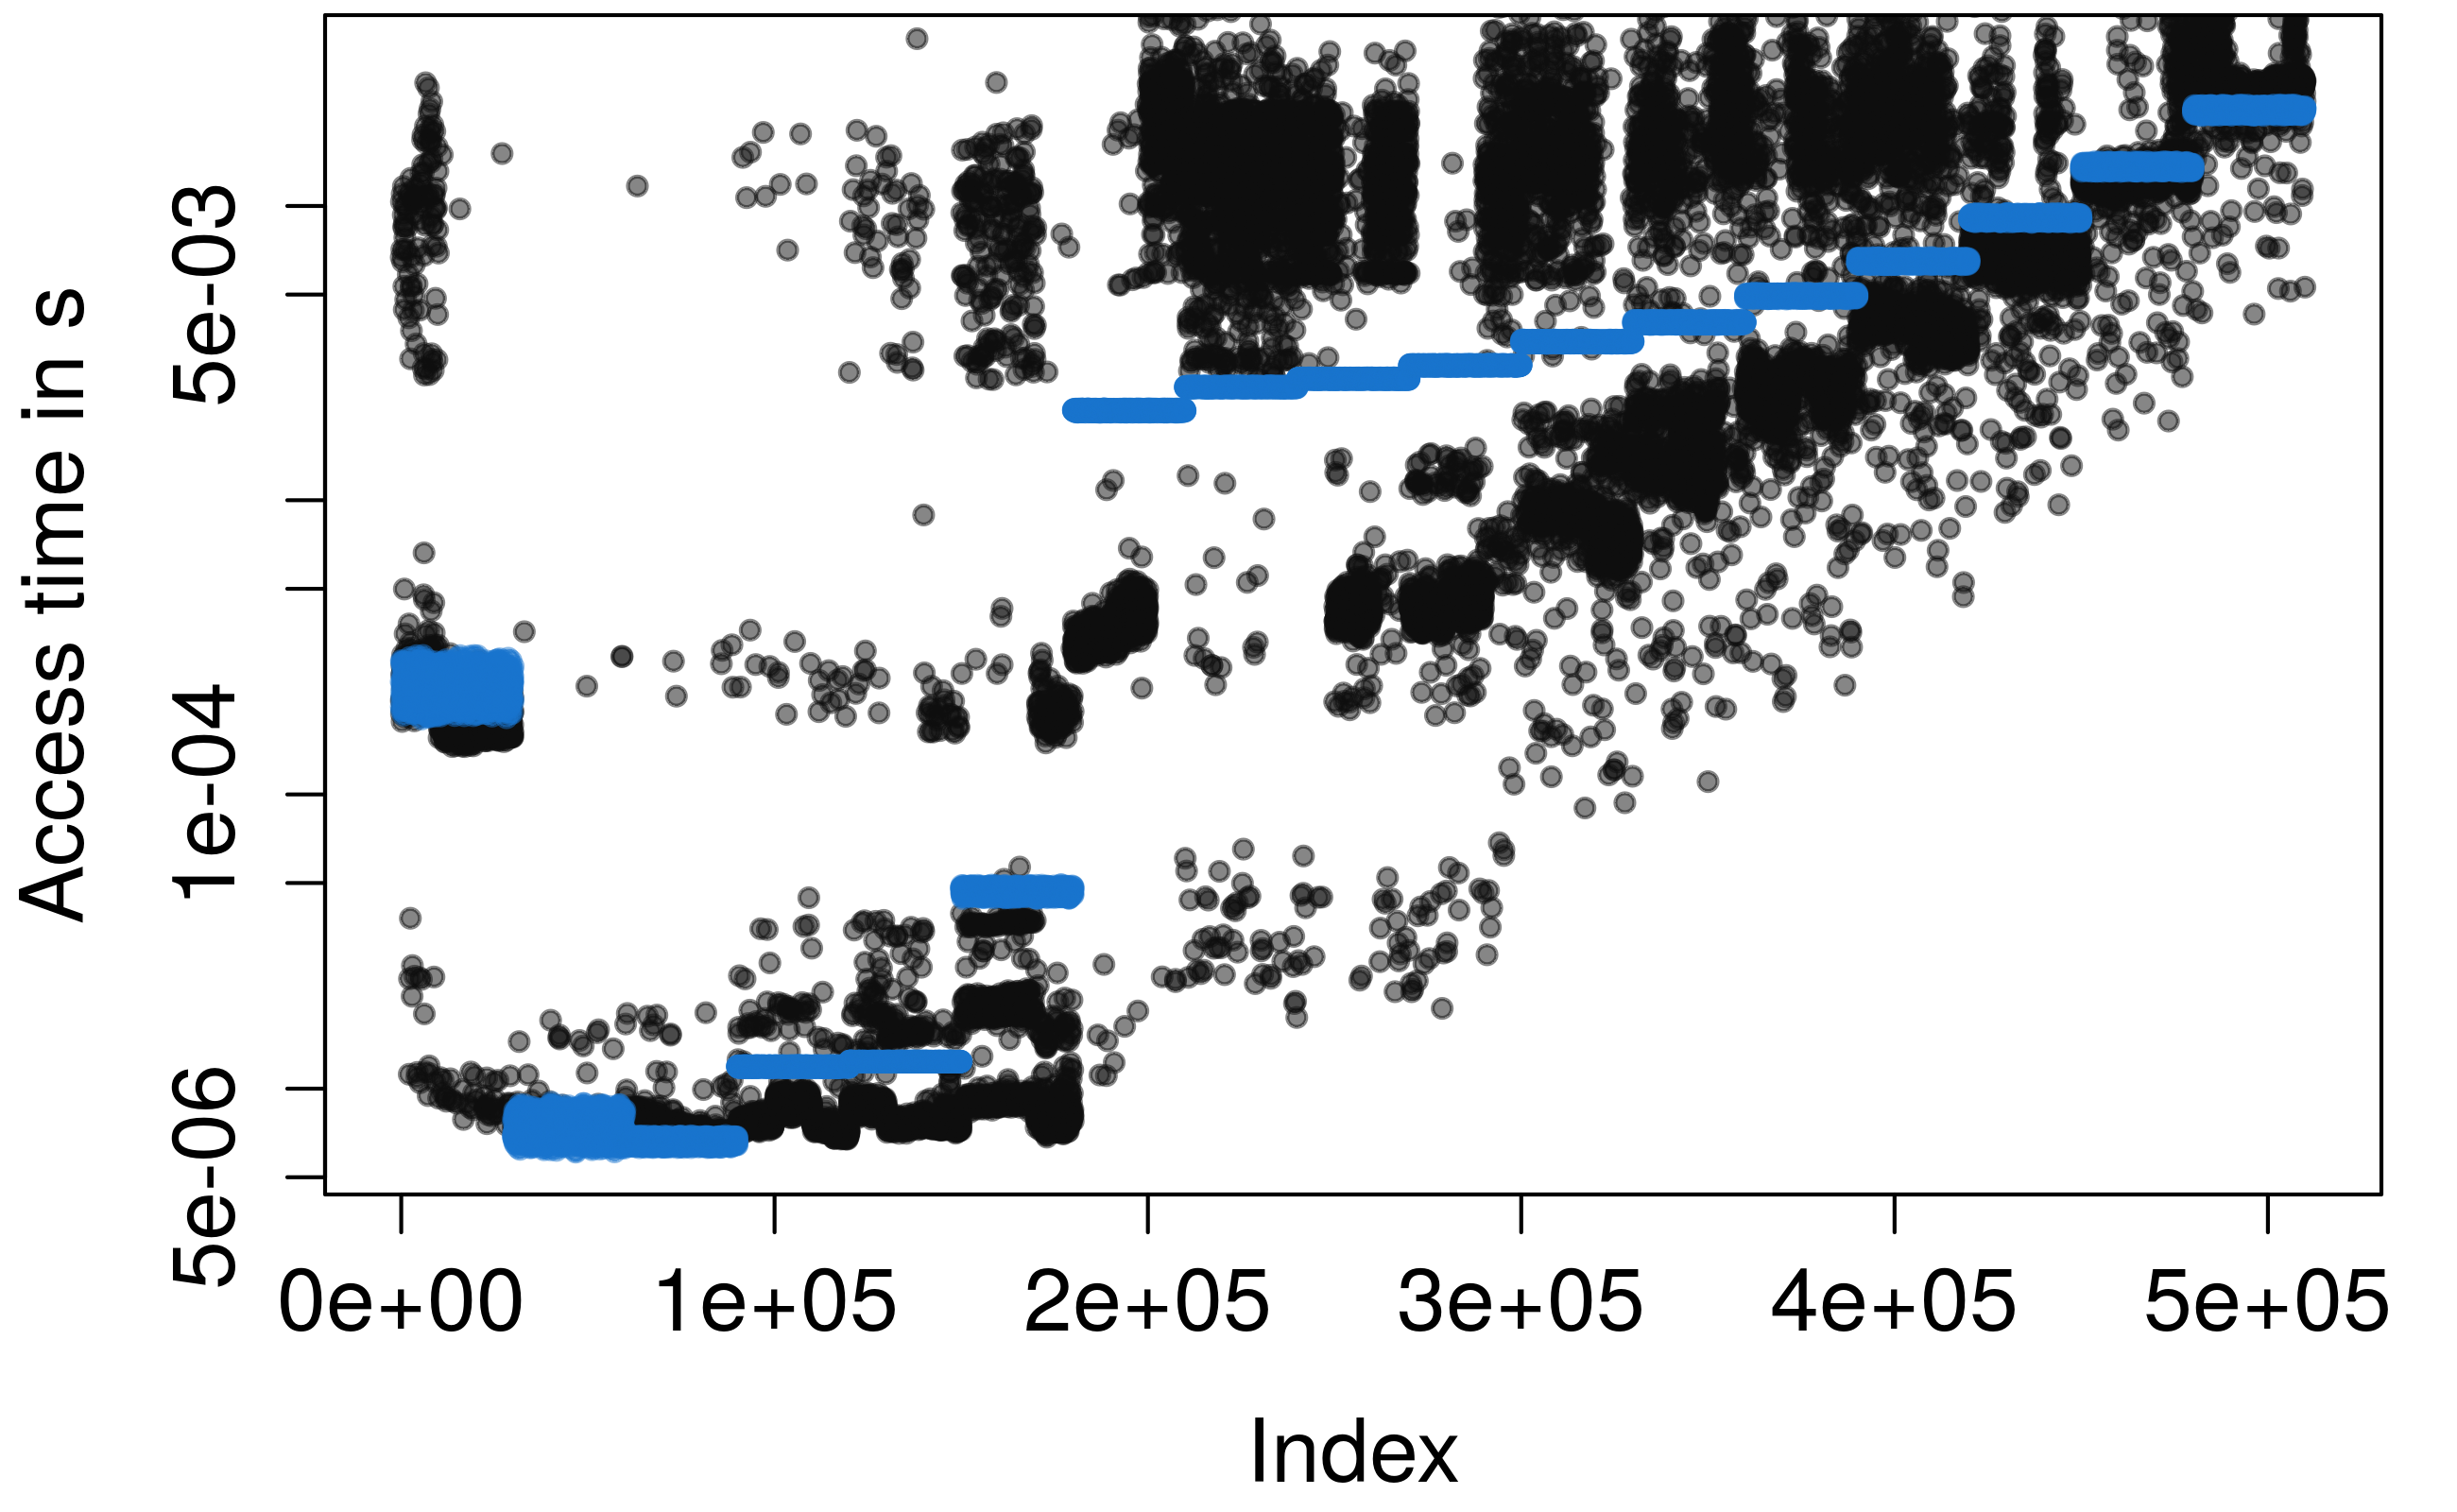
\includegraphics[width=0.48\linewidth]{src/plot_onlyPred_tuple1_Duration_rnd.png}
%		\hfill
%		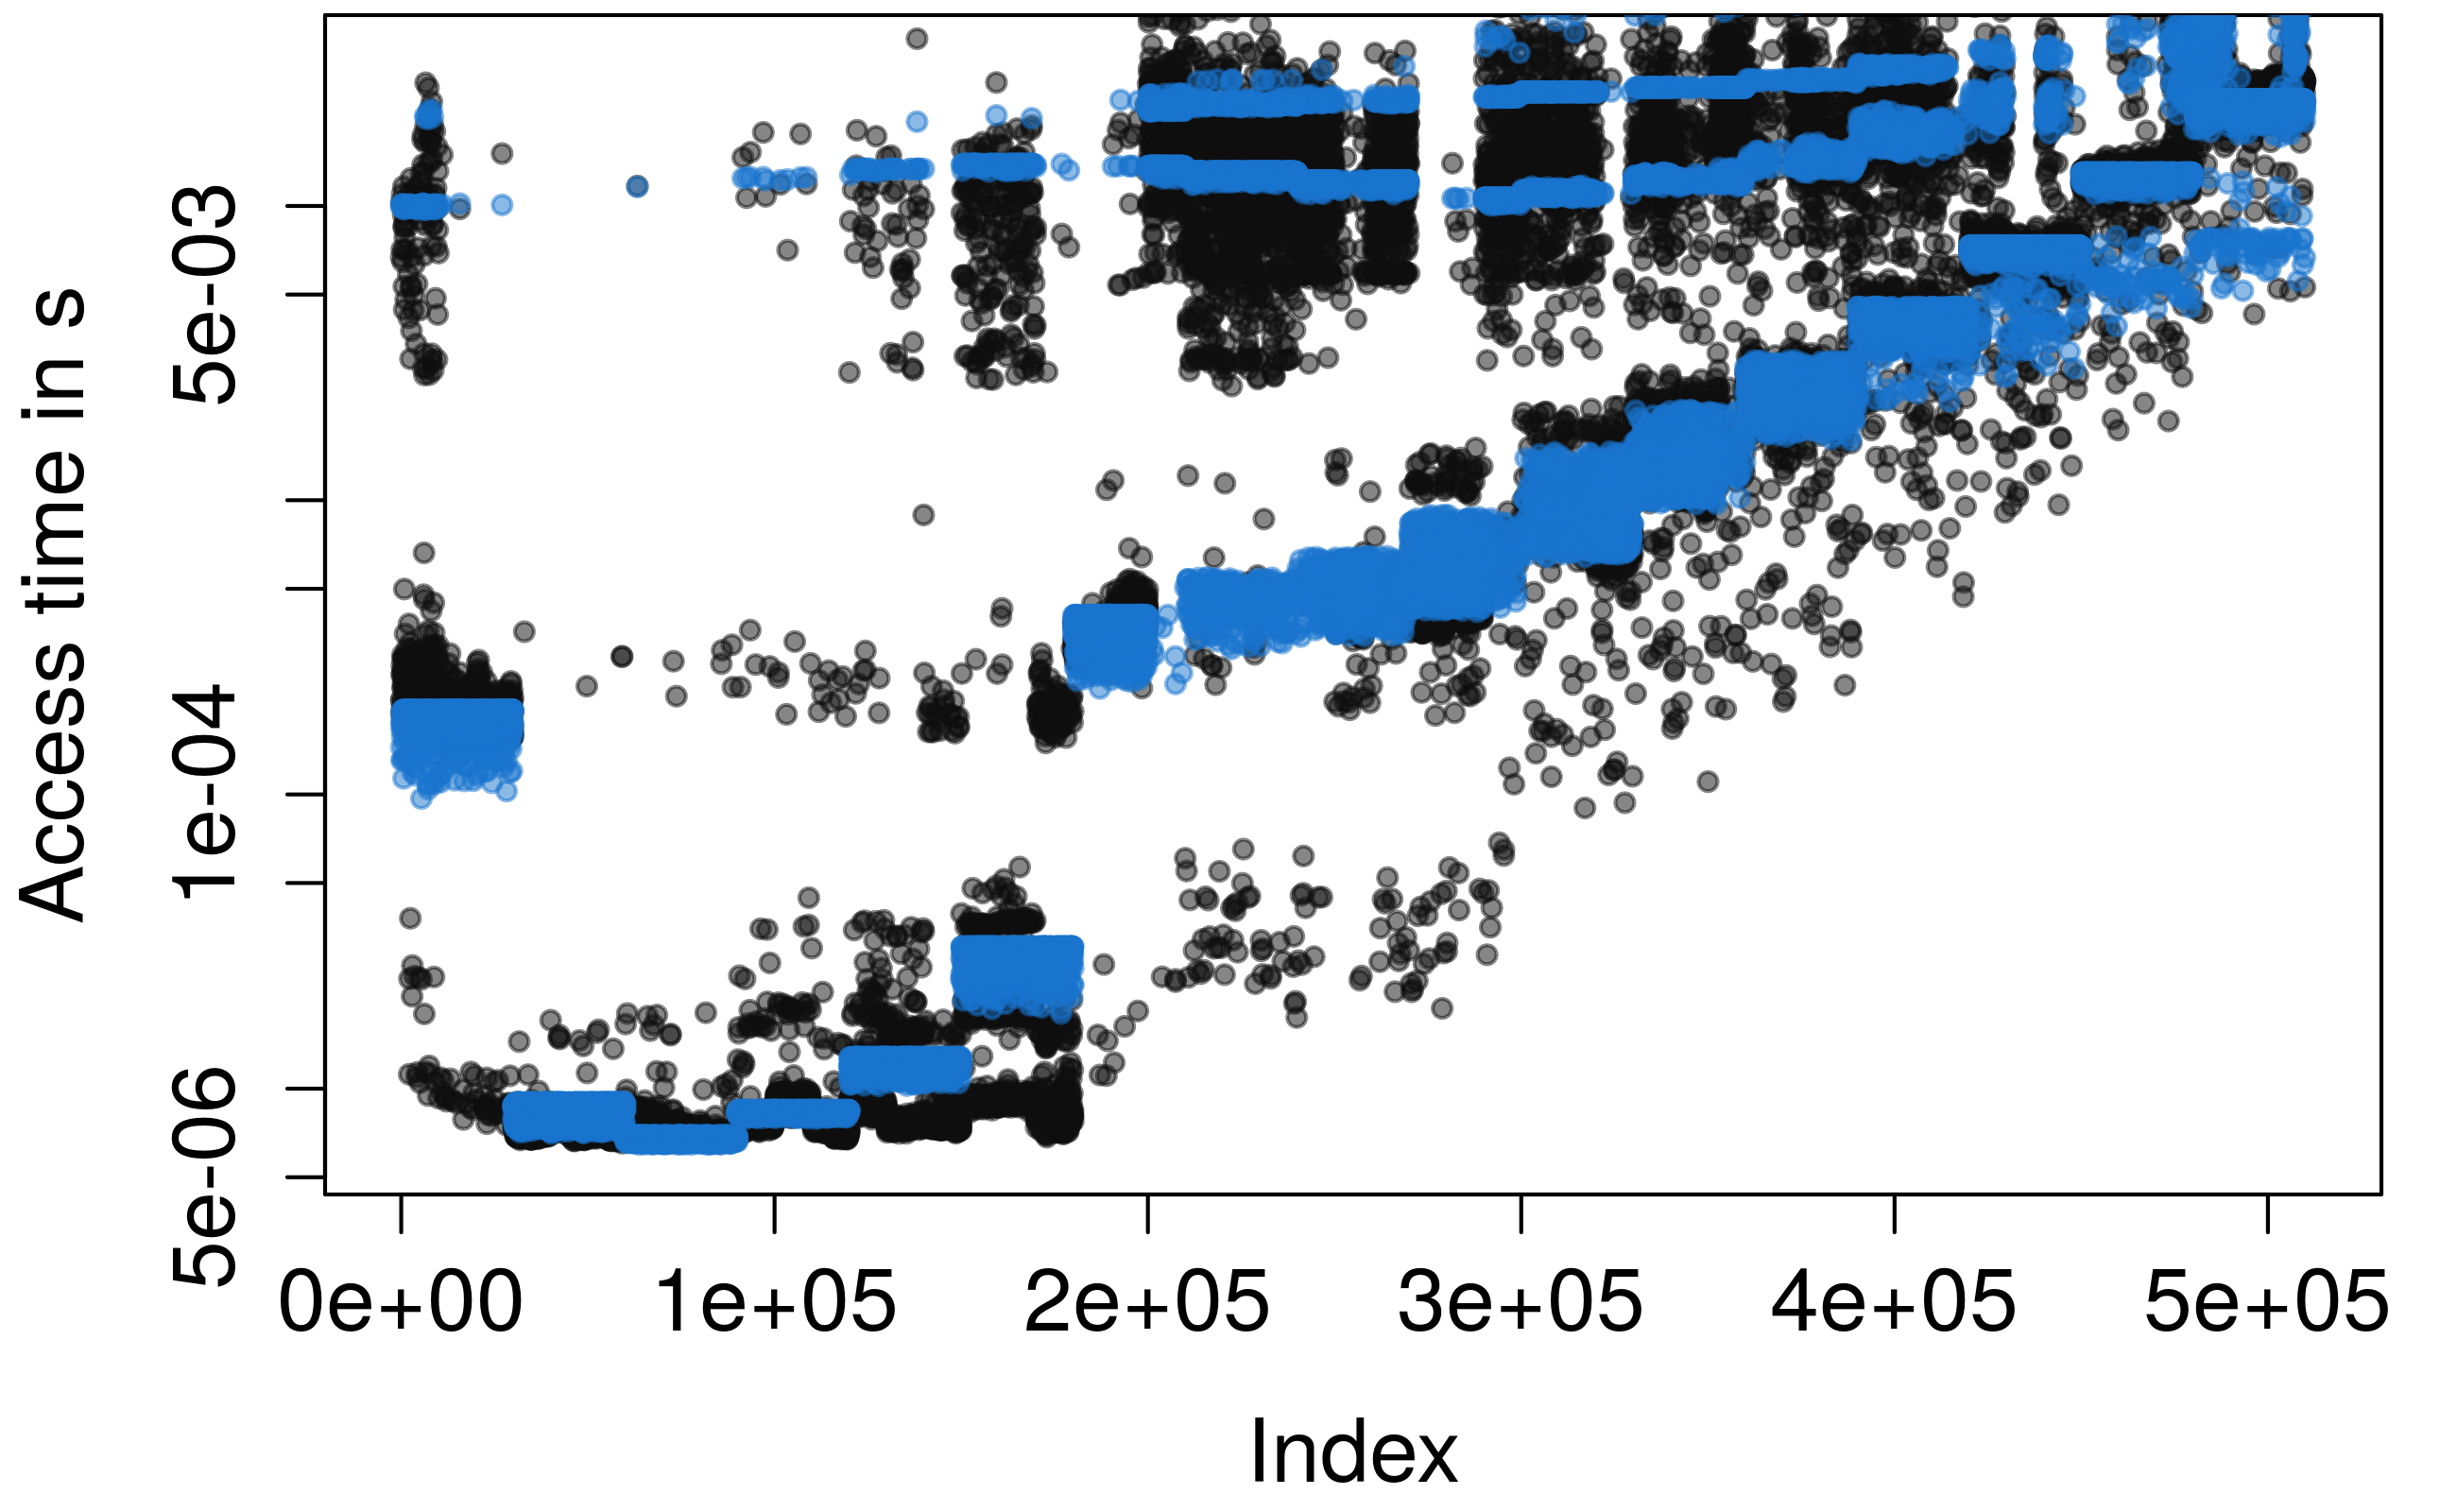
\includegraphics[width=0.48\linewidth]{src/plot_onlyPred_tuple1_with_error_class_from_linreg_Duration_rnd.png}
%		\vspace*{-0.5cm}
%		\caption{Measurements in black; predictions in blue.}
%		\label{preds}
%	\end{figure}
	
\end{block}

%----------------------------------------------------------------------------------------
%	CONCLUSION
%----------------------------------------------------------------------------------------

\vspace*{-1.7cm}
\begin{block}{Conclusion}

	The hypothesis is supported by our data.
	For a good model of HPC storage systems it is therefore necessary to deduce information about I/O-paths.
	If measured access times are available, this can be done with the introduced method.\\
	The method could be a starting point to develop a tool that provides information about I/O-paths used during execution of a program.
	
	%approximates the proportions of used I/O-paths.
	%however further investigations for its practical utilization have to be done.
	

\end{block}


%----------------------------------------------------------------------------------------
%	REFERENCES
%----------------------------------------------------------------------------------------
\vspace*{-0.5cm}
\begin{block}{References}

\nocite{*} % Insert publications even if they are not cited in the poster
\tiny{\bibliographystyle{unsrt}
\bibliography{sample}\vspace{0.75in}}

\end{block}

	\footnotesize
	
	\setbeamercolor{block alerted title}{fg=black,bg=white} % Change the alert block title colors
	\setbeamercolor{block alerted body}{fg=black,bg=white} % Change the alert block body colors
	\vspace*{-2.4cm}
	\begin{exampleblock}{}
		\vspace*{-1cm}
		%\hspace*{5cm}
		\textbf{Contact Information:}
		\vspace*{-0.4cm}
		\begin{itemize}
			%\item Web: \href{http://wr.informatik.uni-hamburg.de}{http://wr.informatik.uni-hamburg.de}
			\item \href{mailto:2schmid@informatik.uni-hamburg.de}{2schmid@informatik.uni-hamburg.de}
			%\item \href{mailto:juliankunkel@googlemail.com}{juliankunkel@googlemail.com}
		\end{itemize}
		
	\end{exampleblock}

%----------------------------------------------------------------------------------------
%	ACKNOWLEDGEMENTS
%----------------------------------------------------------------------------------------

%\setbeamercolor{block title}{fg=red,bg=white} % Change the block title color
%
%\begin{block}{Acknowledgements}
%
%\small{\rmfamily{Nam mollis tristique neque eu luctus. Suspendisse rutrum congue nisi sed convallis. Aenean id neque dolor. Pellentesque habitant morbi tristique senectus et netus et malesuada fames ac turpis egestas.}} \\
%
%\end{block}

%----------------------------------------------------------------------------------------
%	CONTACT INFORMATION
%----------------------------------------------------------------------------------------
%Apricot

%
%\begin{flushright}
%\begin{tabular}{r}
%%
\includegraphics[width=0.2\linewidth]{src/2000px-Unihamburg-logo.png} % & \hfill & \includegraphics[width=0.4\linewidth]{logo.png}
%\end{tabular}
%\end{flushright}

%----------------------------------------------------------------------------------------

\end{column} % End of the 4 column

\end{columns} % End of all the columns in the poster

\end{frame} % End of the enclosing frame

\end{document}
